% Defensa del TFM: 20 diapositivas narradas y una reserva sin numerar.
\documentclass[aspectratio=169,11pt]{beamer}

\usepackage{fontspec}
\usefonttheme{professionalfonts}
\setmainfont{lmroman10-regular.otf}[
  BoldFont=lmroman10-bold.otf,
  ItalicFont=lmroman10-italic.otf,
  BoldItalicFont=lmroman10-bolditalic.otf
]
\setsansfont{lmsans10-regular.otf}[
  BoldFont=lmsans10-bold.otf,
  ItalicFont=lmsans10-oblique.otf,
  BoldItalicFont=lmsans10-boldoblique.otf
]
\usepackage[spanish,es-tabla,es-noquoting]{babel}
\usepackage{amsmath,amssymb,booktabs,graphicx,tikz}
\usetikzlibrary{arrows.meta,positioning,calc}

\definecolor{navy}{HTML}{16324F}
\definecolor{teal}{HTML}{007C83}
\definecolor{gold}{HTML}{C58B00}
\definecolor{rojo}{HTML}{B33A3A}
\definecolor{verde}{HTML}{2C7A4B}
\definecolor{slate}{HTML}{5D6D7E}
\definecolor{light}{HTML}{E8EEF2}

\setbeamertemplate{navigation symbols}{}
\setbeamercolor{background canvas}{bg=white}
\setbeamercolor{normal text}{fg=black!85}
\setbeamercolor{frametitle}{fg=navy}
\setbeamercolor{itemize item}{fg=teal}
\setbeamerfont{frametitle}{size=\Large,series=\bfseries}
\setbeamertemplate{itemize item}{\raisebox{0.15ex}{\rule{0.7ex}{0.7ex}}}

\newcommand{\acto}{navy}
\newcommand{\setacto}[1]{\renewcommand{\acto}{#1}}
\setbeamertemplate{frametitle}{%
  \vspace*{0.35cm}
  \begin{minipage}{\linewidth}
    \usebeamerfont{frametitle}\usebeamercolor[fg]{frametitle}\insertframetitle\\[0.16cm]
    {\color{\acto}\rule{2.2cm}{1.6pt}}
  \end{minipage}}
\setbeamertemplate{footline}{%
  \hfill{\small\color{slate}\insertframenumber/20}\hspace*{0.65cm}\vspace*{0.25cm}}

\newcommand{\cifra}[2]{%
  \begin{center}
    {\fontsize{22}{24}\selectfont\color{navy}\textbf{#1}}\\[0.25em]
    {\small\color{slate}#2}
  \end{center}}
\newcommand{\cifracolor}[3]{%
  \begin{center}
    {\fontsize{22}{24}\selectfont\color{#3}\textbf{#1}}\\[0.25em]
    {\small\color{slate}#2}
  \end{center}}
\newcommand{\matiz}[1]{%
  \par\medskip\noindent
  \colorbox{light}{\parbox{\dimexpr\linewidth-2\fboxsep\relax}{%
    \small{\color{gold}\textbf{Límite.}}~#1}}}
\newcommand{\rankic}{\text{rank-IC}}
% GENERADO por latex/scripts/export_study_assets.py. No editar a mano.
% Las rutas y los identificadores se verifican internamente; el PDF solo consume macros.
\newcommand{\NumPredictores}{68}
\newcommand{\NumParametrosCatalogo}{33}
\newcommand{\NumDiagnosticos}{75}
\newcommand{\RankICSeleccion}{0,1067}
\newcommand{\RankICRisk}{0,1201}
\newcommand{\CohortesSeleccion}{117}
\newcommand{\FraccionICPositiva}{76,1\%}
\newcommand{\ICIRSeleccion}{0,833}
\newcommand{\TNeweyWest}{3,33}
\newcommand{\PValorPermutacion}{0,0001}
\newcommand{\NumPermutaciones}{9.999}
\newcommand{\ProbabilidadDSR}{0,573}
\newcommand{\RankICReservado}{0,0364}
\newcommand{\CohortesReservadas}{6}
\newcommand{\FraccionICReservadaPositiva}{66,7\%}
\newcommand{\GapShareRisk}{47,8\%}
\newcommand{\RangeShareRisk}{33,7\%}
\newcommand{\DosVariablesRisk}{81,5\%}
\newcommand{\NumCarteras}{1.440}
\newcommand{\IRModelo}{0,312}
\newcommand{\ExcesoModelo}{2,12\%}
\newcommand{\TurnoverModelo}{2,42}
\newcommand{\MDDModelo}{25,21\%}
\newcommand{\IRModeloReservado}{-1,795}
\newcommand{\ExcesoModeloReservado}{-12,23\%}
\newcommand{\IRCartera}{0,841}
\newcommand{\ExcesoCartera}{5,91\%}
\newcommand{\TurnoverCartera}{1,35}
\newcommand{\MDDCartera}{22,83\%}
\newcommand{\BeatRateCartera}{100\%}
\newcommand{\IRCarteraReservado}{0,109}
\newcommand{\ExcesoCarteraReservado}{0,24\%}
\newcommand{\TurnoverCarteraReservado}{0,35}
\newcommand{\MDDCarteraReservado}{16,08\%}
\newcommand{\BeatRateCarteraReservado}{50\%}
\newcommand{\AnosCarteraReservada}{1,41}
\newcommand{\PosicionesCartera}{8}
\newcommand{\EfectivoModelo}{25\%}
\newcommand{\EfectivoCartera}{10\%}
\newcommand{\TenenciaModelo}{half horizon}
\newcommand{\TenenciaCartera}{full horizon}
\newcommand{\DerivaModelo}{0,25}
\newcommand{\DerivaCartera}{0,40}
\newcommand{\InfluenciaPosiciones}{0,208}
\newcommand{\InfluenciaTenencia}{0,164}
\newcommand{\InfluenciaEfectivo}{0,139}
\newcommand{\InfluenciaCobertura}{0,076}
\newcommand{\InfluenciaDeriva}{0,017}
\newcommand{\InfluenciaPesos}{0,005}
\newcommand{\CosteAdoptado}{30}
\newcommand{\CosteEquilibrio}{294}
\newcommand{\NumAccionesCartera}{42}
\newcommand{\NumEpisodiosCartera}{49}
\newcommand{\MedianaMesesTenencia}{15}
\newcommand{\ContribucionAAPL}{27,8\%}


\title{Aprendizaje automático aplicado a la selección de acciones}
\author{Adrián Núñez}
\date{\today}

\begin{document}

% 1 · 0:20
{\setbeamertemplate{footline}{}
\begin{frame}[plain]
  \vspace{1.0cm}
  \hspace*{0.45cm}\begin{minipage}{0.90\linewidth}
    {\color{navy}\rule{2.2cm}{2pt}}\\[0.8cm]
    {\fontsize{24}{28}\selectfont\color{navy}\textbf{Aprendizaje automático aplicado\\a la selección de acciones}}\\[0.55cm]
    {\large\color{slate}Medición honesta del aprendizaje fuera de muestra}\\[1.35cm]
    {\large\textbf{Adrián Núñez}}\\[0.2cm]
    {\small\color{slate}Trabajo Fin de Máster · Defensa}
  \end{minipage}
\end{frame}}
\note{[0:20] Este trabajo separa dos preguntas que suelen confundirse: si el modelo aprende a
ordenar acciones y si una cartera real consigue cobrar esa ordenación. La defensa sigue esa cadena.}

% 2 · 0:45
\begin{frame}{Batir al mercado es un listón excepcionalmente alto}
  \vspace{-0.15cm}
  \begin{center}
    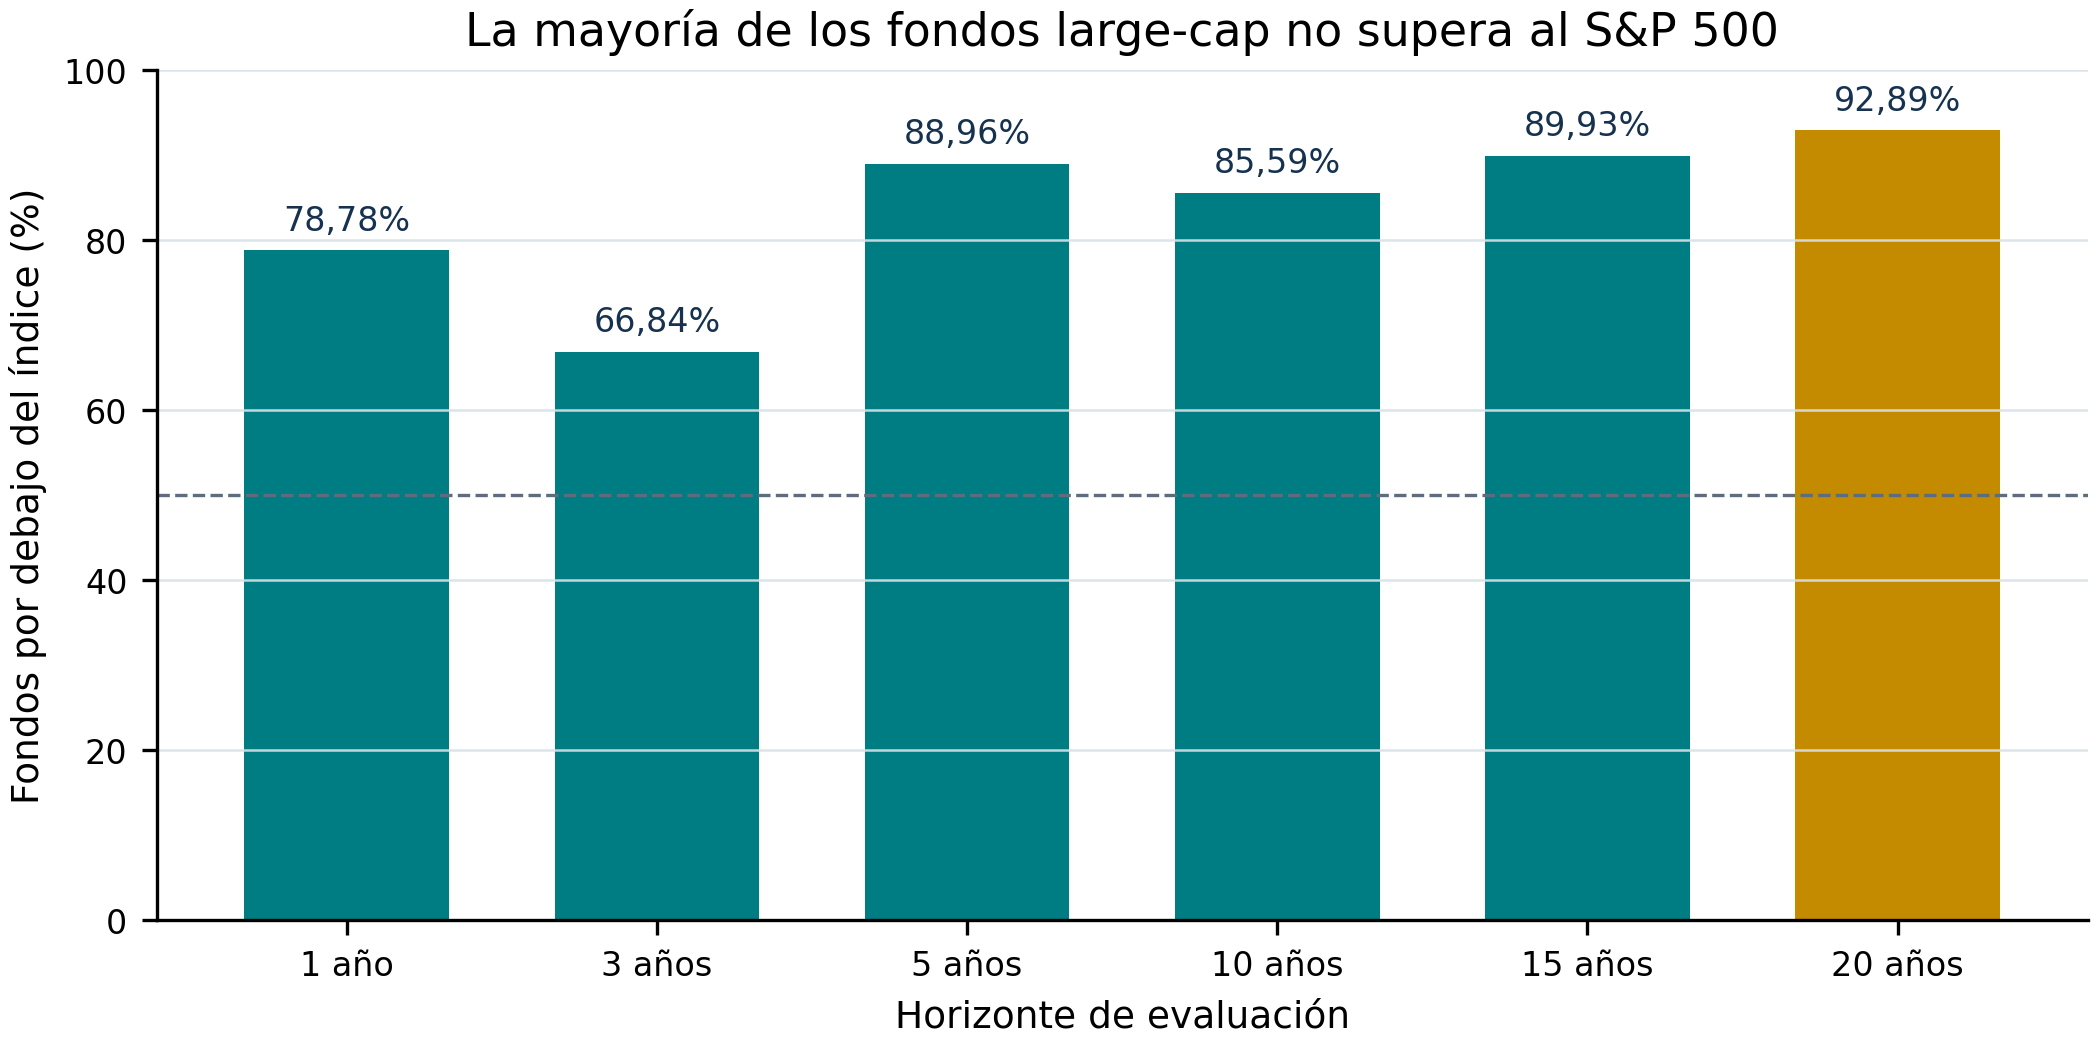
\includegraphics[height=0.58\textheight,keepaspectratio]{assets/f01_spiva_horizontes.png}
  \end{center}
  \vspace{-0.22cm}
  \matiz{No hay progresión estrictamente monótona, pero a veinte años el 92,89\,\% queda por debajo.}
\end{frame}
\note{[0:45] Antes de formular los objetivos conviene fijar el listón económico. SPIVA compara
fondos estadounidenses de gran capitalización con el S\&P 500: la mayoría no lo supera en ninguno
de los horizontes publicados y a veinte años falla el 92,89 por ciento. No es una serie monótona,
pero sí persistentemente alta. El segundo objetivo intenta cobrar señal en ese entorno.
[Sources]
- https://www.spglobal.com/spdji/en/documents/spiva/spiva-us-year-end-2025.pdf — Report 1a,
  All Large-Cap Funds frente al S\&P 500, rentabilidad absoluta; datos a 31-12-2025.}

% 3 · 0:50
\begin{frame}{Dos objetivos, dos métricas}
  \vspace{0.35cm}
  \begin{columns}[t,onlytextwidth]
    \begin{column}{0.47\textwidth}
      {\color{navy}\Large\textbf{1 · Señal}}\\[0.35cm]
      {\large ¿Aprende el sistema a \textbf{ordenar} acciones fuera de muestra?}\\[0.55cm]
      {\color{slate}\textbf{Decisión:} Rank-IC robusto.}
    \end{column}
    \begin{column}{0.47\textwidth}
      {\color{teal}\Large\textbf{2 · Cartera}}\\[0.35cm]
      {\large ¿Importa \textbf{cómo se materializa} ese orden en posiciones?}\\[0.55cm]
      {\color{slate}\textbf{Decisión:} Information Ratio.}
    \end{column}
  \end{columns}
  \vspace{0.65cm}
  \begin{center}
    \colorbox{light}{\parbox{0.90\linewidth}{\centering\large
      Ordenar bien y ganar dinero son capacidades relacionadas, no equivalentes.}}
  \end{center}
\end{frame}
\note{[0:50] El objetivo uno se decide exclusivamente por Rank-IC, que mide si el orden predicho
coincide con el retorno futuro. El objetivo dos se abre después, con la señal congelada, y mide la
calidad relativa de la cartera. Esta separación evita elegir modelo por una cartera afortunada.}

% 3 · 0:55
\begin{frame}{Cinco especialistas alimentan un meta-agente}
  \vspace{0.2cm}
  \begin{center}
  \begin{tikzpicture}[node distance=0.42cm and 0.55cm,>=Latex,
    box/.style={draw=navy,rounded corners,minimum width=2.15cm,minimum height=0.75cm,
      align=center,fill=light,font=\small\bfseries}]
    \node[box] (q) {quality};
    \node[box,right=of q] (v) {value};
    \node[box,right=of v] (g) {growth};
    \node[box,right=of g] (m) {momentum};
    \node[box,right=of m] (r) {risk};
    \node[box,draw=teal,fill=teal!10,below=1.0cm of g,minimum width=3.2cm] (meta) {meta-agente};
    \node[box,draw=gold,fill=gold!10,below=0.8cm of meta,minimum width=3.2cm] (rank) {ranking transversal};
    \foreach \x in {q,v,g,m,r} \draw[->,color=slate] (\x.south) -- (meta.north);
    \draw[->,thick,color=teal] (meta) -- (rank);
  \end{tikzpicture}
  \end{center}
  \vspace{0.4cm}
  \begin{columns}[c,onlytextwidth]
    \begin{column}{0.47\textwidth}\cifra{\NumPredictores}{predictores declarados}\end{column}
    \begin{column}{0.47\textwidth}\cifra{\NumParametrosCatalogo}{parámetros del catálogo}\end{column}
  \end{columns}
\end{frame}
\note{[0:55] Cada especialista recibe un bloque disjunto de información y produce un ranking. El
meta aprende pesos usando solo cohortes cerradas. Los 68 predictores no son los 33 parámetros del
catálogo; además existen 73 diagnósticos porque se auditan columnas derivadas.}

% 4 · 0:55
\begin{frame}{Cada decisión usa solo información disponible entonces}
  \vspace{0.35cm}
  \begin{center}
  \begin{tikzpicture}[>=Latex,thick]
    \draw[->,color=slate] (0,0) -- (12.4,0);
    \foreach \x/\lab in {1/periodo fiscal,4/publicación,7/snapshot,11/cierre de etiqueta}{
      \draw[navy] (\x,-0.16)--(\x,0.16);
      \node[align=center,below=0.28cm,font=\small] at (\x,0) {\lab};}
    \draw[->,color=teal,line width=2pt] (4,0.7) -- (7,0.7);
    \node[above,font=\small\bfseries,text=teal] at (5.5,0.7) {lag de ejecución};
    \draw[->,color=gold,line width=2pt] (7,1.45) -- (11,1.45);
    \node[above,font=\small\bfseries,text=gold] at (9,1.45) {retorno futuro};
  \end{tikzpicture}
  \end{center}
  \vspace{0.75cm}
  \begin{itemize}\setlength{\itemsep}{0.4em}
    \item Composición histórica del S\&P 500, no la actual.
    \item Fundamentales fechados por publicación; precios unidos hacia atrás.
    \item Una etiqueta entra en entrenamiento cuando su horizonte ya terminó.
  \end{itemize}
\end{frame}
\note{[0:55] El periodo fiscal no equivale a la fecha en que el mercado conocía la cifra. Por eso
se usa filing date y un lag adicional. El retorno futuro solo sirve como etiqueta cuando ha cerrado.
La cobertura histórica sigue siendo imperfecta y se declara como limitación.}

% 5 · 1:00
\begin{frame}{Las decisiones terminan antes de abrir la era reservada}
  \vspace{0.45cm}
  \begin{center}
  \begin{tikzpicture}[>=Latex,node distance=0.35cm]
    \node[draw,rounded corners,fill=navy!9,minimum width=2.3cm,minimum height=0.9cm] (t) {Temporal};
    \node[draw,rounded corners,fill=navy!9,right=of t,minimum width=2.3cm,minimum height=0.9cm] (rep) {Representación};
    \node[draw,rounded corners,fill=navy!9,right=of rep,minimum width=2.3cm,minimum height=0.9cm] (mod) {Modelo};
    \node[draw,rounded corners,fill=navy!9,right=of mod,minimum width=2.3cm,minimum height=0.9cm] (meta) {Meta};
    \node[draw,rounded corners,fill=teal!12,below=0.75cm of rep,minimum width=3.2cm,minimum height=0.9cm] (freeze) {Señal congelada};
    \node[draw,rounded corners,fill=gold!14,right=0.8cm of freeze,minimum width=3.6cm,minimum height=0.9cm] (port) {Carteras diagnósticas};
    \draw[->] (t)--(rep); \draw[->] (rep)--(mod); \draw[->] (mod)--(meta);
    \draw[->] (meta.south) |- (freeze.east); \draw[->] (freeze)--(port);
  \end{tikzpicture}
  \end{center}
  \vspace{0.55cm}
  \begin{columns}[c,onlytextwidth]
    \begin{column}{0.48\textwidth}\cifra{2015--2024}{selección: todas las decisiones}\end{column}
    \begin{column}{0.48\textwidth}\cifracolor{2025--2026}{reservada: ninguna decisión}{gold}\end{column}
  \end{columns}
\end{frame}
\note{[1:00] Tres Model Studies recorren de forma secuencial las fases predictivas. Después se
congela el ganador y se abre el Portfolio Study. La rejilla se calcula con la serie truncada en
2024. La ventana 2025--2026 solo se consulta al final.}

% 6 · 0:50
\begin{frame}{Rank-IC mide el orden, no la rentabilidad}
  \vspace{0.35cm}
  \begin{columns}[c,onlytextwidth]
    \begin{column}{0.45\textwidth}
      \[
        \rankic_t=\rho_{\mathrm{Spearman}}
        \bigl(\widehat{s}_{i,t},r_{i,t\rightarrow t+h}\bigr)
      \]
    \end{column}
    \begin{column}{0.49\textwidth}
      \begin{itemize}\setlength{\itemsep}{0.55em}
        \item $>0$: arriba rinde mejor que abajo.
        \item No exige calibrar euros ni porcentajes.
        \item No depende del tamaño ni de la rotación de la cartera.
      \end{itemize}
    \end{column}
  \end{columns}
  \vspace{0.65cm}
  \begin{center}
    {\large\color{navy}\textbf{Por eso puede mantenerse positivo mientras una cartera pierde.}}
  \end{center}
\end{frame}
\note{[0:50] Rank-IC es la correlación de rangos entre la puntuación y el retorno futuro. Permite
evaluar la señal antes de decidir cuántas acciones comprar. Una cartera solo consume una parte del
ranking y añade costes, concentración y reglas de salida.}

% 7 · 1:05
\begin{frame}{El meta aprende a concentrarse, pero no supera al mejor especialista}
  \begin{columns}[c,onlytextwidth]
    \begin{column}{0.62\textwidth}
      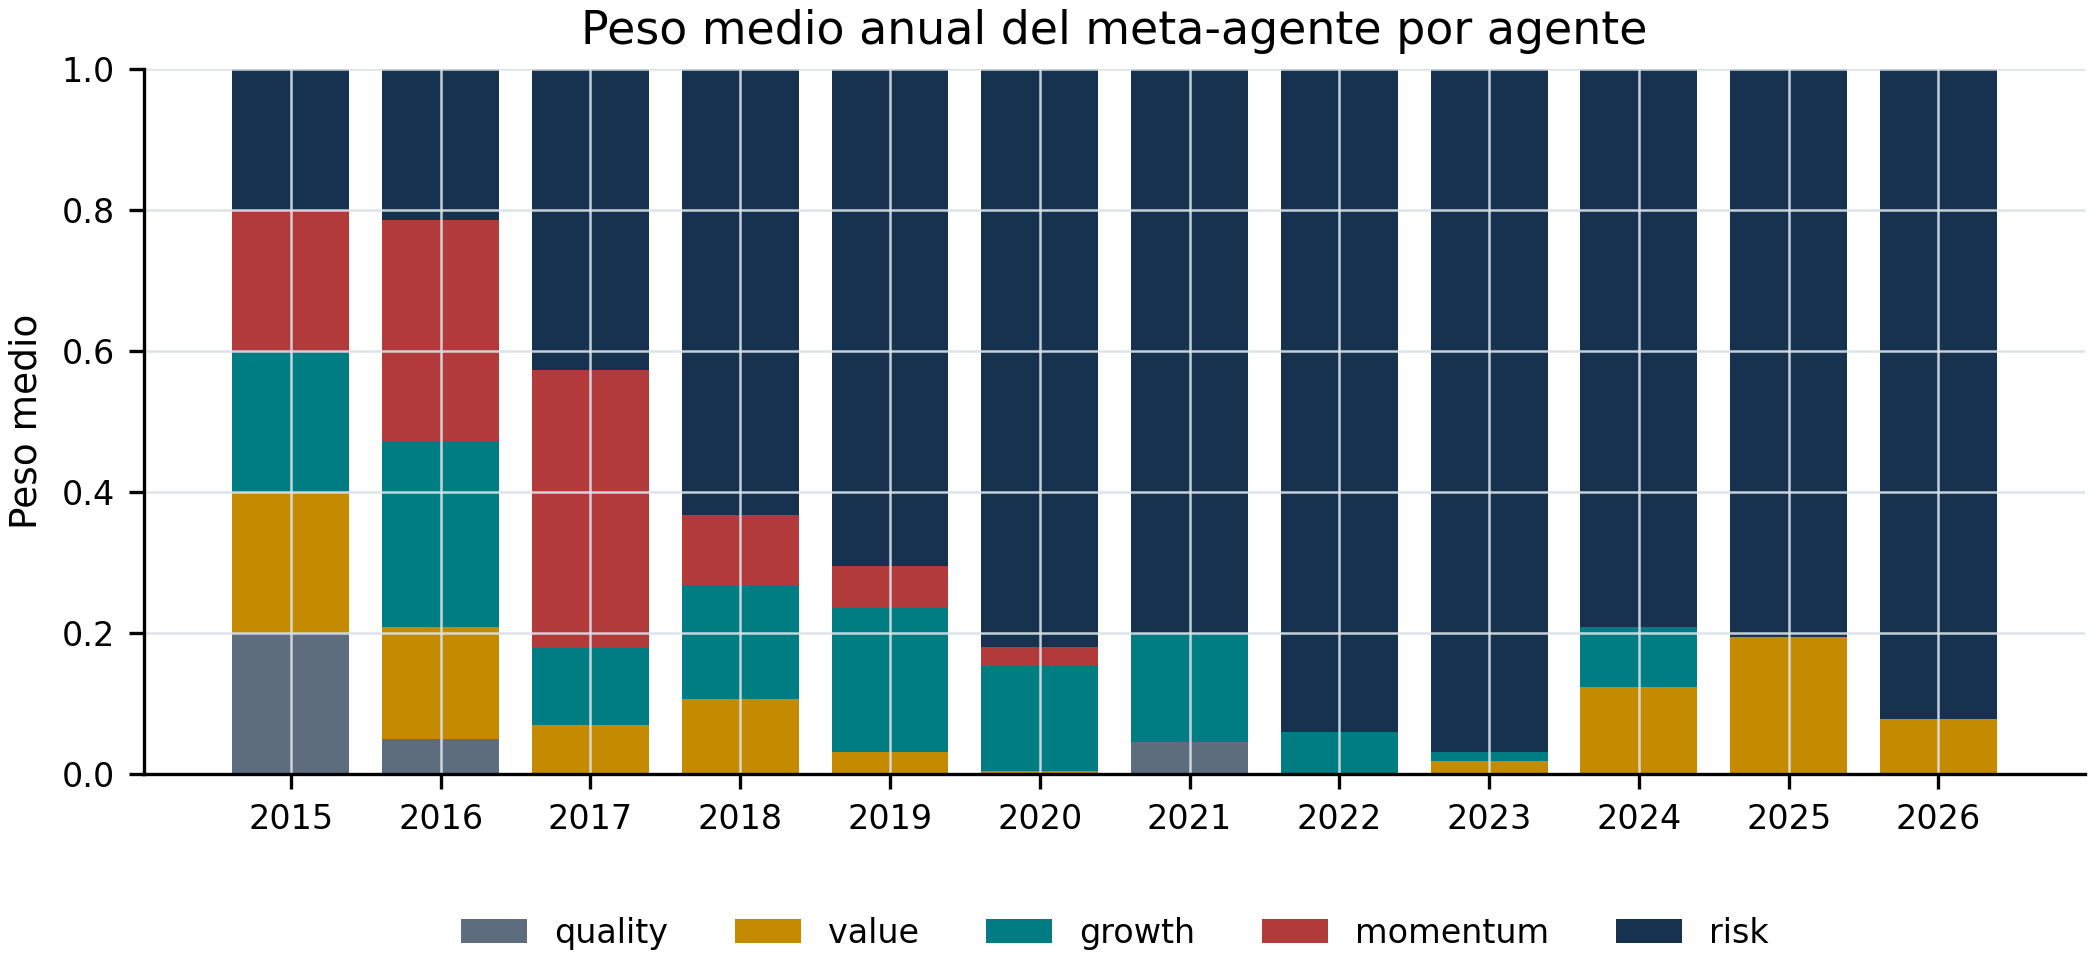
\includegraphics[width=\linewidth]{assets/f05_pesos_anual.png}
    \end{column}
    \begin{column}{0.34\textwidth}
      \cifra{\RankICRisk}{Rank-IC de risk}
      \vspace{0.25cm}
      \cifra{\RankICSeleccion}{Rank-IC del meta}
    \end{column}
  \end{columns}
  \matiz{El sistema aprende a elegir al especialista dominante; estos datos no demuestran que la
  arquitectura de cinco agentes sea necesaria.}
\end{frame}
\note{[1:05] Los pesos parten iguales y se concentran progresivamente en risk, usando solo cohortes
cerradas. Eso demuestra aprendizaje del meta frente al promedio equiponderado. Pero risk solo llega
a 0,1201 y supera al meta, 0,1067. La conclusión no puede ser que combinar cinco agentes sea mejor.}

% 8 · 0:50
\begin{frame}{Dos variables explican el \DosVariablesRisk{} del liderazgo de \texttt{risk}}
  \begin{columns}[c,onlytextwidth]
    \begin{column}{0.62\textwidth}
      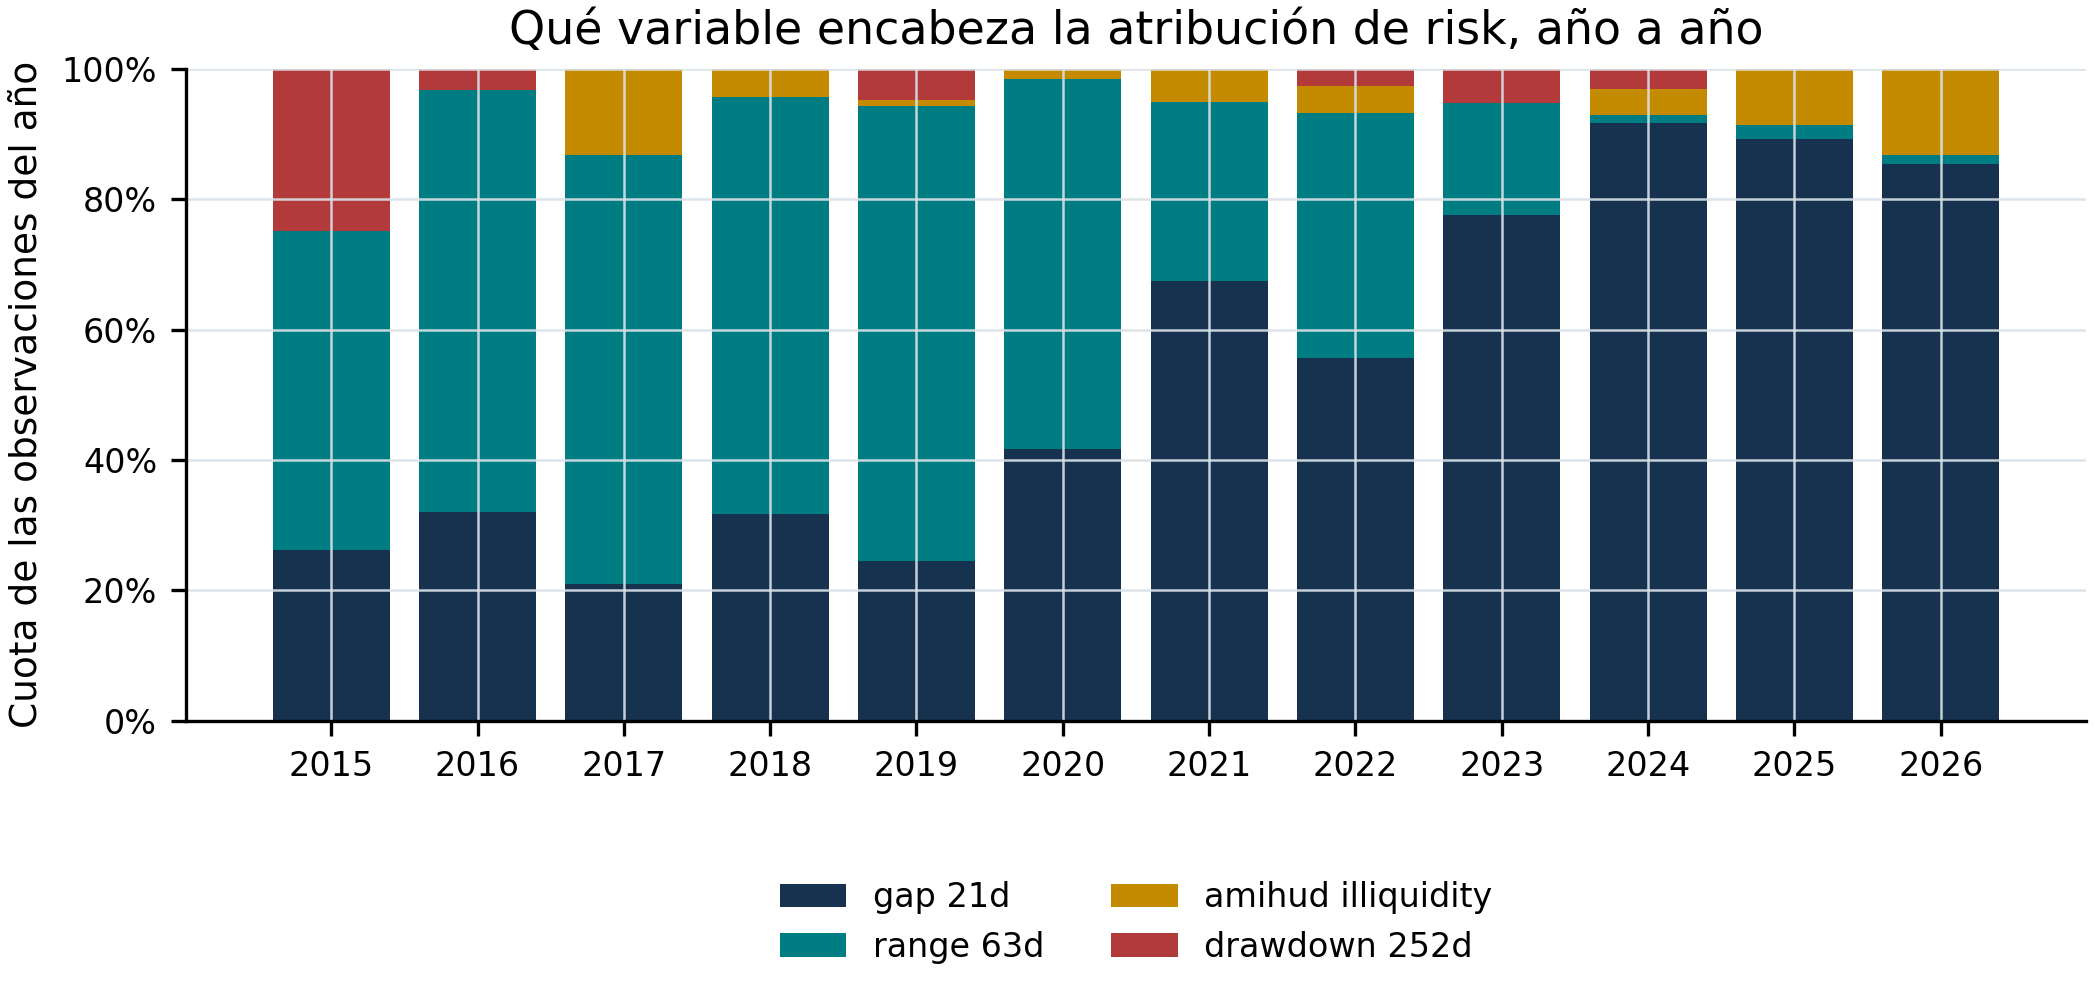
\includegraphics[width=\linewidth]{assets/f05_atribucion_anual.png}
    \end{column}
    \begin{column}{0.34\textwidth}
      \cifra{\GapShareRisk}{gap\_21d}
      \vspace{0.2cm}
      \cifra{\RangeShareRisk}{range\_63d}
    \end{column}
  \end{columns}
  \matiz{La atribución describe microestructura de precio; no identifica por sí sola una causa económica.}
\end{frame}
\note{[0:50] Gap de 21 días y rango de 63 encabezan conjuntamente el 81,5 por ciento. El resultado
no es simplemente beta o volatilidad anual. Puede reflejar liquidez o microestructura; el TFM lo
describe, no lo convierte en una explicación causal.}

% 9 · 1:00
\begin{frame}{La señal es positiva, pero cambia de intensidad entre eras}
  \begin{columns}[c,onlytextwidth]
    \begin{column}{0.64\textwidth}
      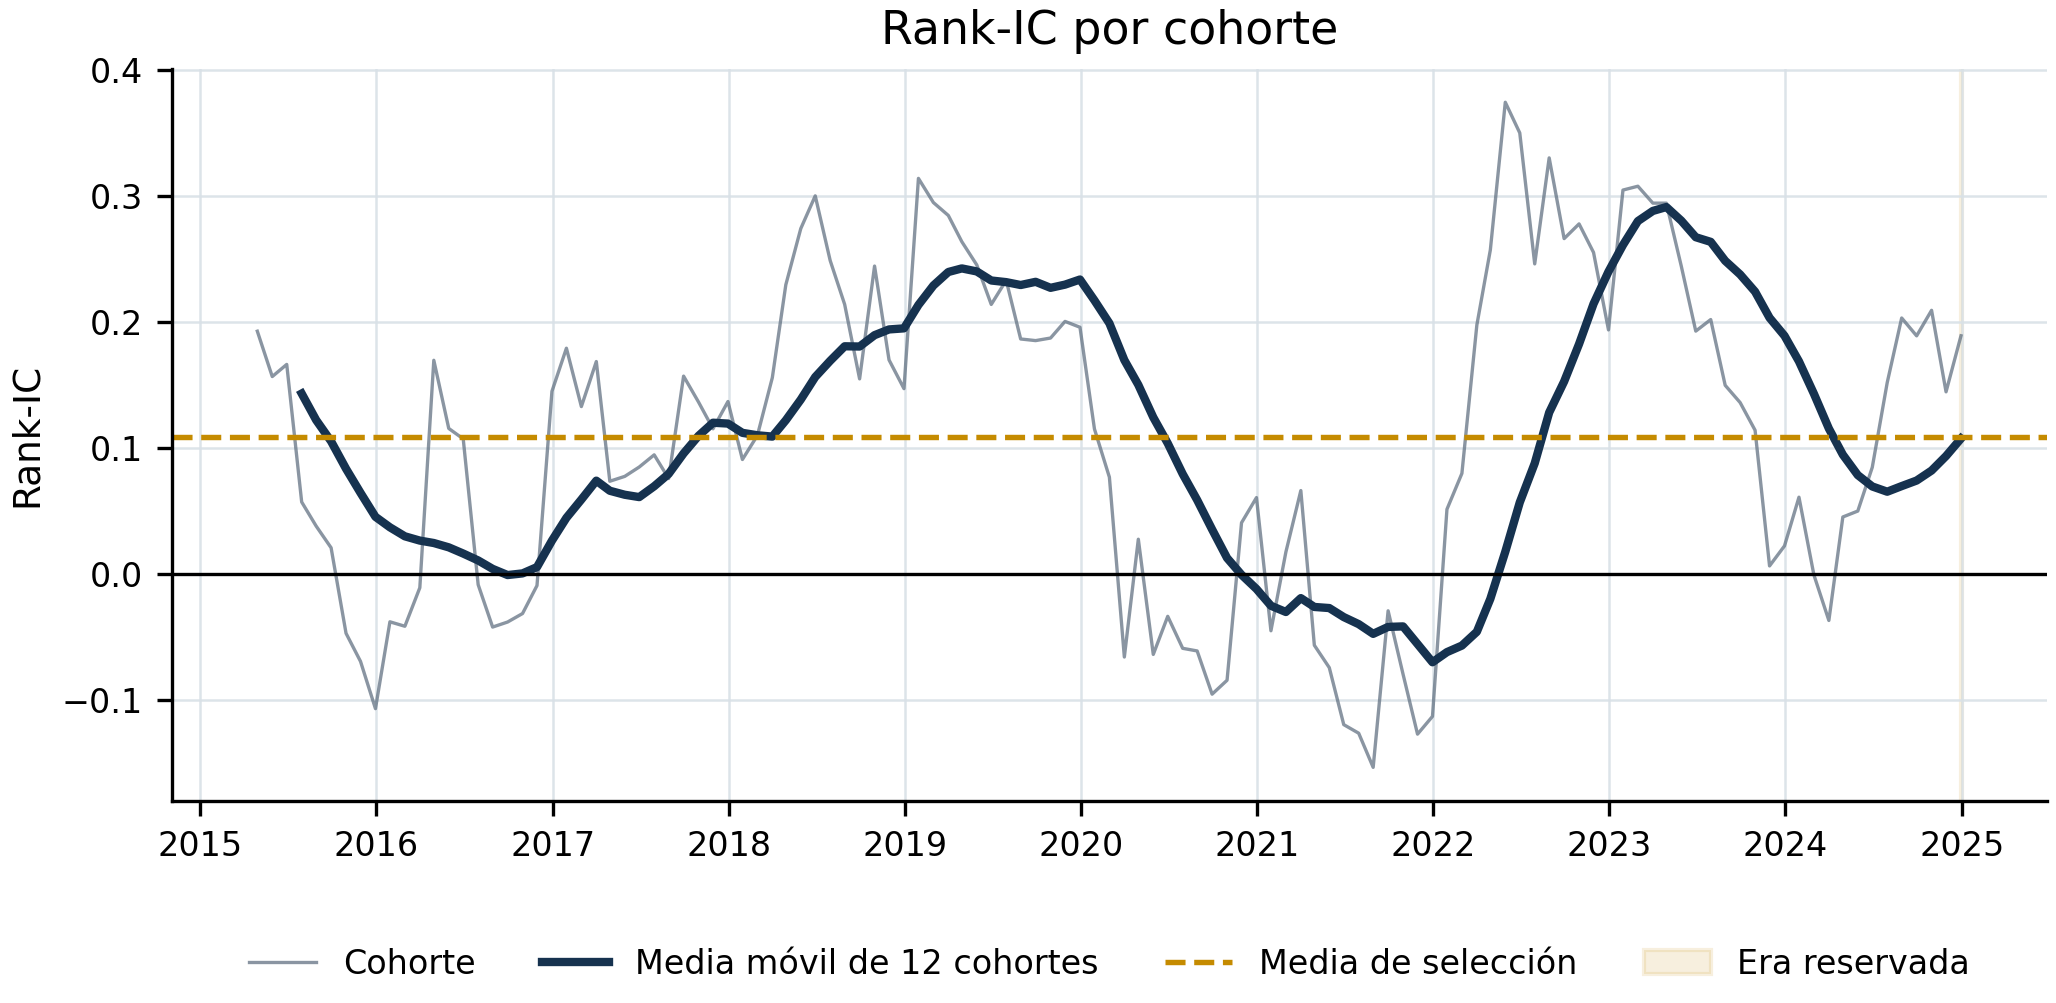
\includegraphics[width=\linewidth]{assets/f07_rankic_serie.png}
    \end{column}
    \begin{column}{0.32\textwidth}
      \cifra{\RankICSeleccion}{media 2015--2024}
      \vspace{0.15cm}
      \cifra{\FraccionICPositiva}{cohortes positivas}
      \vspace{0.15cm}
      \cifracolor{\RankICReservado}{era reservada}{gold}
    \end{column}
  \end{columns}
  \matiz{La era reservada aporta solo \CohortesReservadas{} cohortes cerradas.}
\end{frame}
\note{[1:00] En selección hay 117 cohortes, Rank-IC 0,1067 y 76,1 por ciento positivas. La media
reservada sigue positiva, 0,0364, pero con seis cohortes. La señal no es homogénea y la ventana final
no tiene potencia para una confirmación fuerte.}

% 10 · 0:55
\begin{frame}{Siete contrastes respaldan la señal; uno limita la rentabilidad}
  \begin{columns}[c,onlytextwidth]
    \begin{column}{0.58\textwidth}
      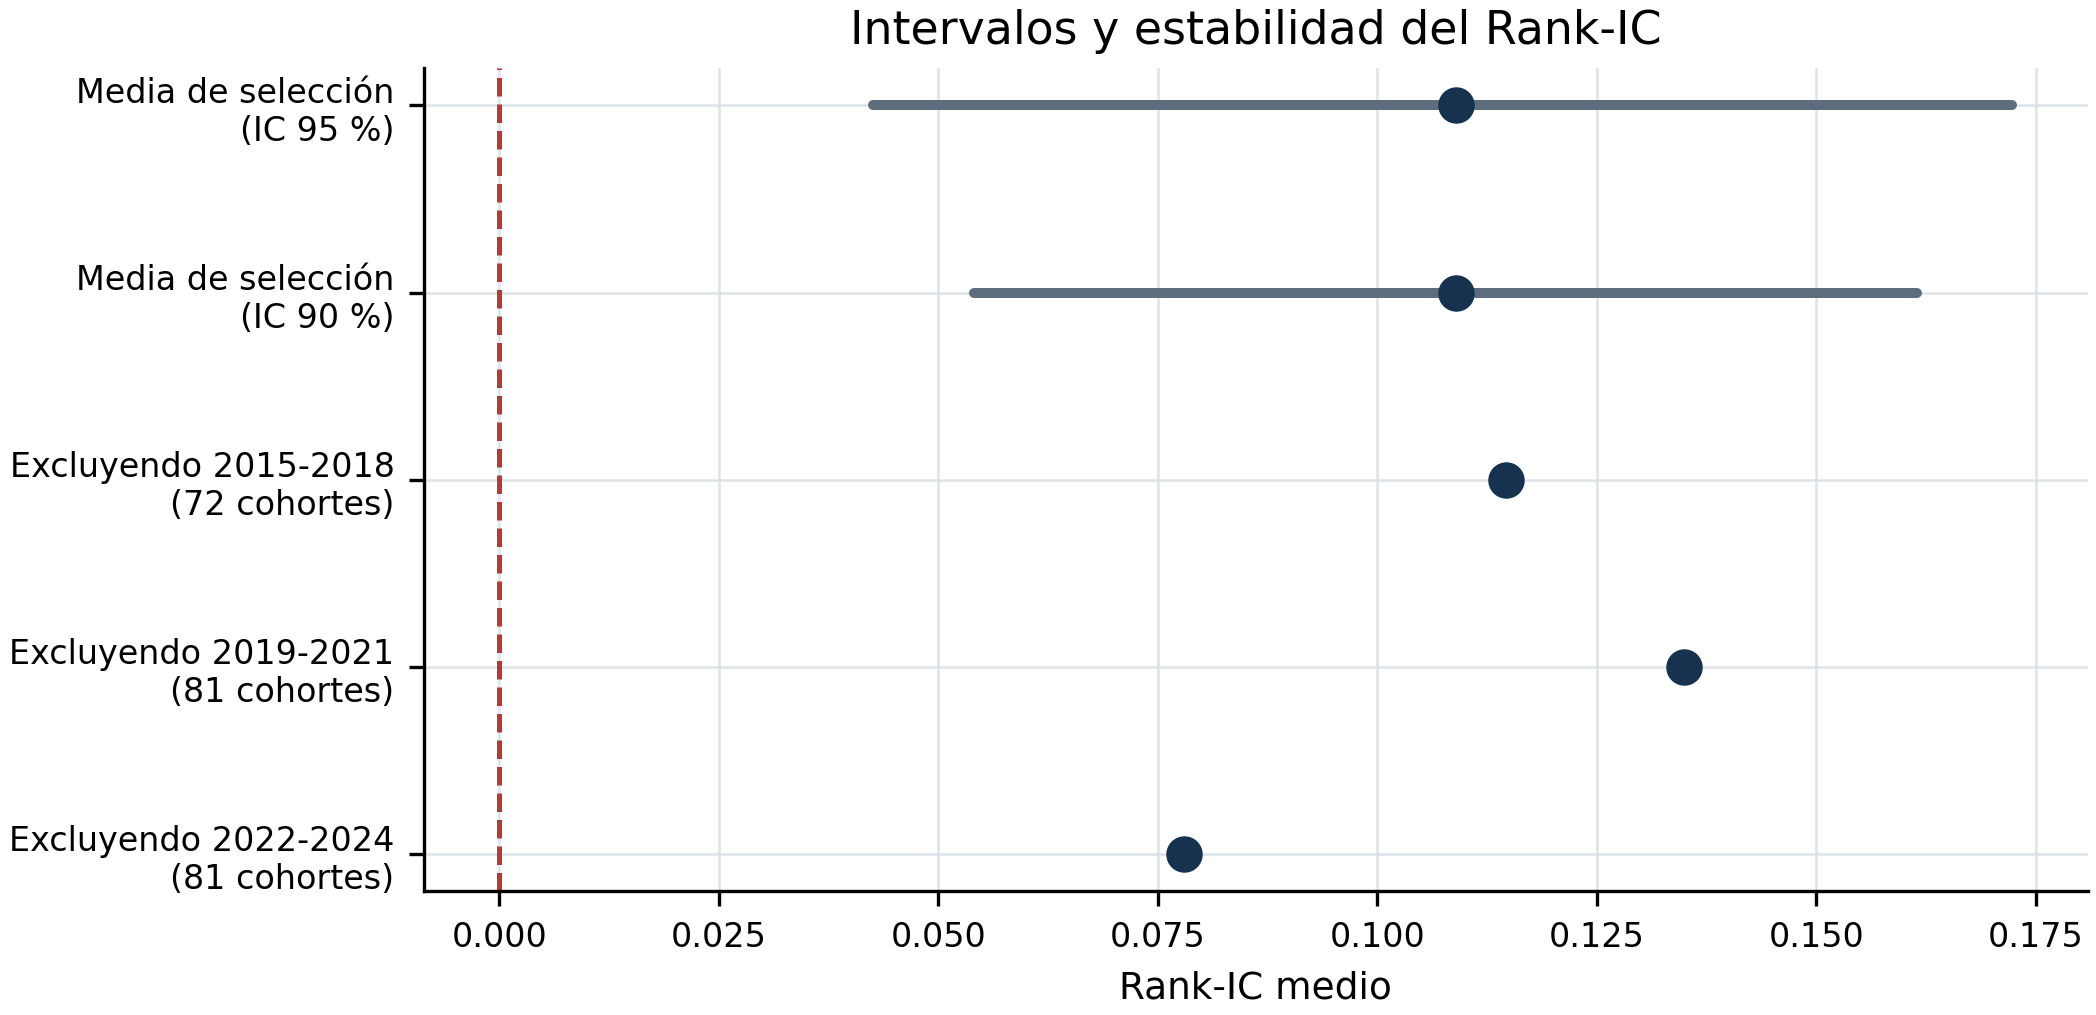
\includegraphics[width=\linewidth]{assets/f07_bootstrap.png}
    \end{column}
    \begin{column}{0.38\textwidth}
      \begin{itemize}\setlength{\itemsep}{0.35em}
        \item $t_{NW}=\TNeweyWest{}$
        \item permutación: $p=\PValorPermutacion{}$
        \item eras, semillas y placebos: favorables
        \item \textbf{Deflated Sharpe: \ProbabilidadDSR{}}
      \end{itemize}
    \end{column}
  \end{columns}
  \matiz{La evidencia de ordenación es más fuerte que la de rentabilidad ajustada por selección.}
\end{frame}
\note{[0:55] El bootstrap por bloques excluye cero, ninguna era sostiene por sí sola el resultado y
ninguna de 9.999 permutaciones alcanza la señal. El contraste que falla es Deflated Sharpe: 0,573.
No afirmo una rentabilidad ajustada por multiplicidad.}

% 11 · 1:05
\begin{frame}{La cadena mejora el orden dentro y no cobra fuera}
  \begin{columns}[c,onlytextwidth]
    \begin{column}{0.62\textwidth}
      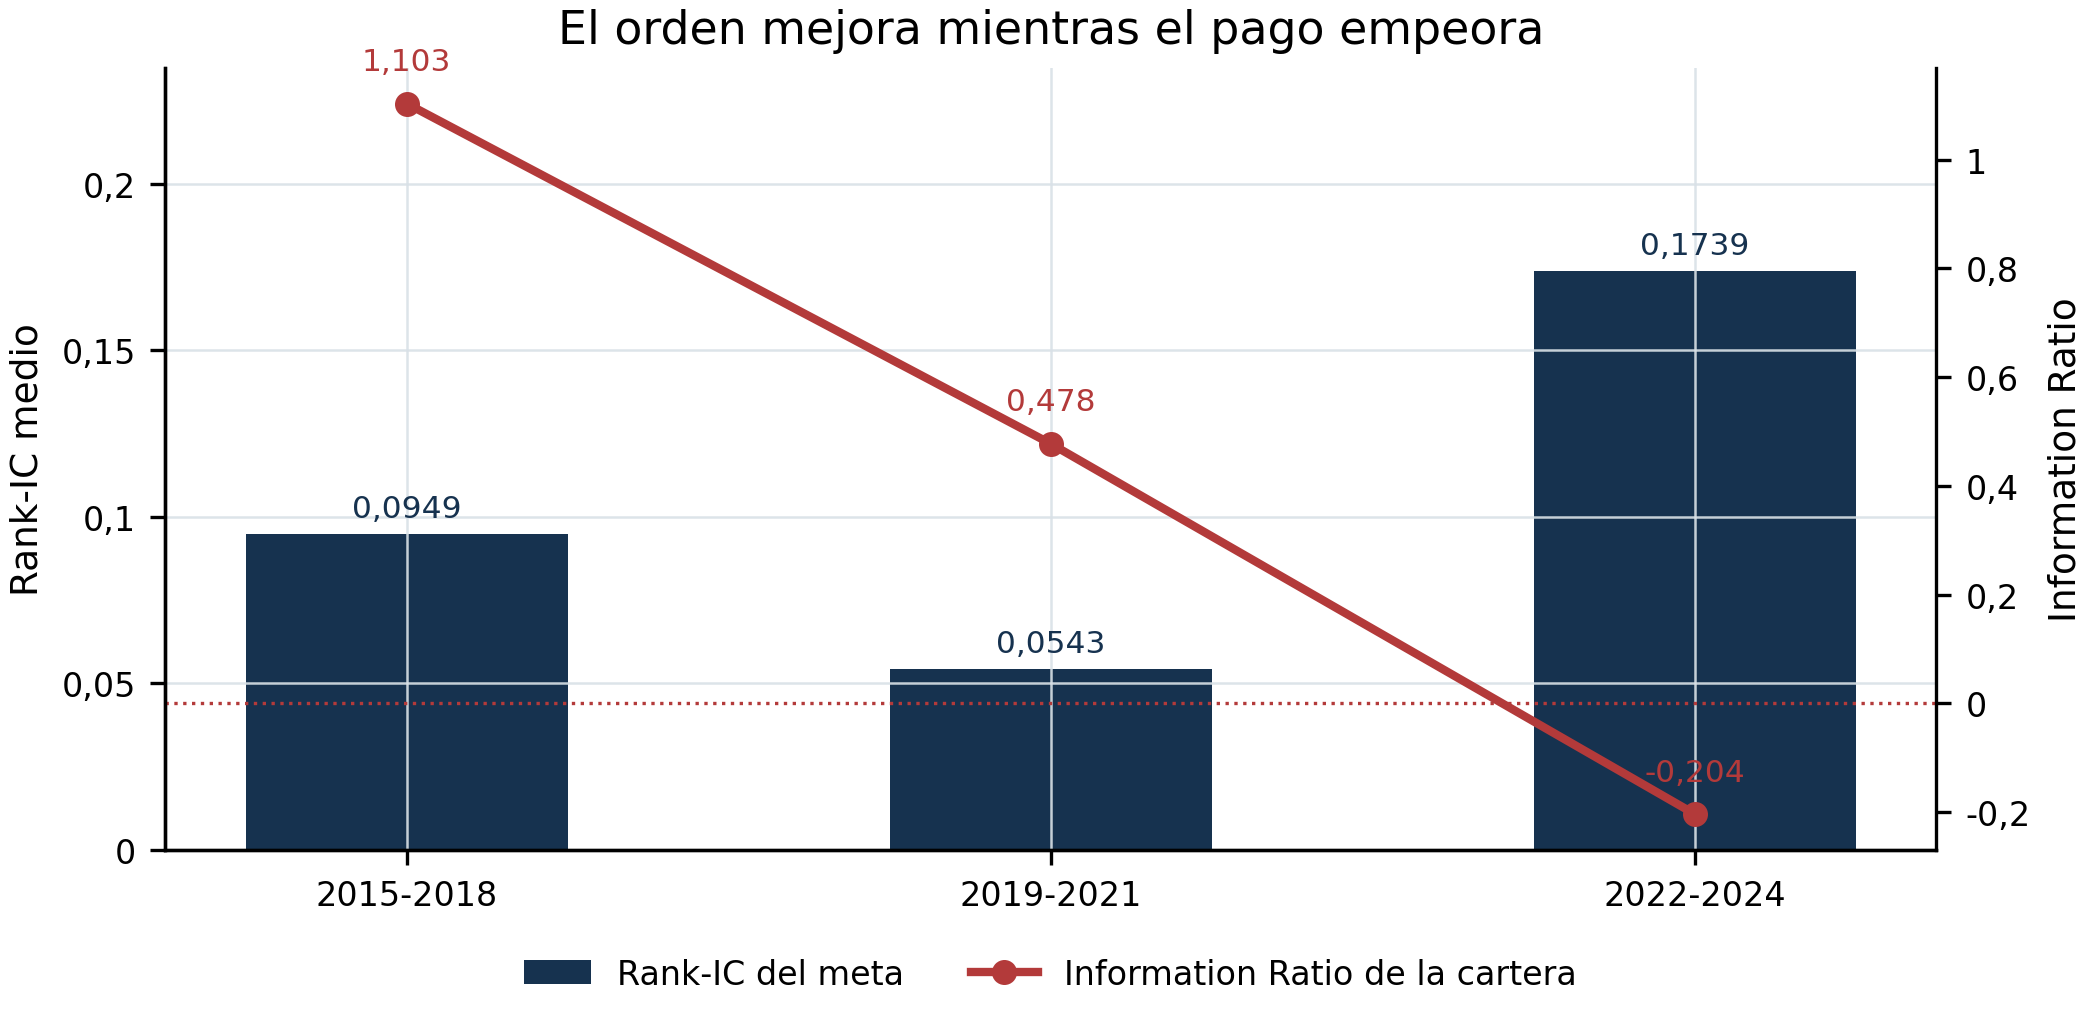
\includegraphics[width=\linewidth]{assets/f06_orden_vs_pago.png}
    \end{column}
    \begin{column}{0.34\textwidth}
      {\large\color{navy}\textbf{Rank-IC}}\\
      mejora en la era reciente.\\[0.55cm]
      {\large\color{rojo}\textbf{Information Ratio}}\\
      empeora con la cartera original.
    \end{column}
  \end{columns}
  \matiz{La divergencia identifica la implementación como palanca observable; no prueba que toda
  debilidad económica sea ajena a la señal.}
\end{frame}
\note{[1:05] Esta es la tensión central. El orden transversal mejora en la era más reciente, mientras
el pago económico de la cartera original cae. Eso contradice una explicación simple basada solo en
peor cobertura temprana y justifica estudiar la cartera sin reabrir el modelo.}

\setacto{teal}
\begin{frame}{Tres reglas concentran casi toda la sensibilidad de la cartera}
  \begin{columns}[c,onlytextwidth]
    \begin{column}{0.66\textwidth}
      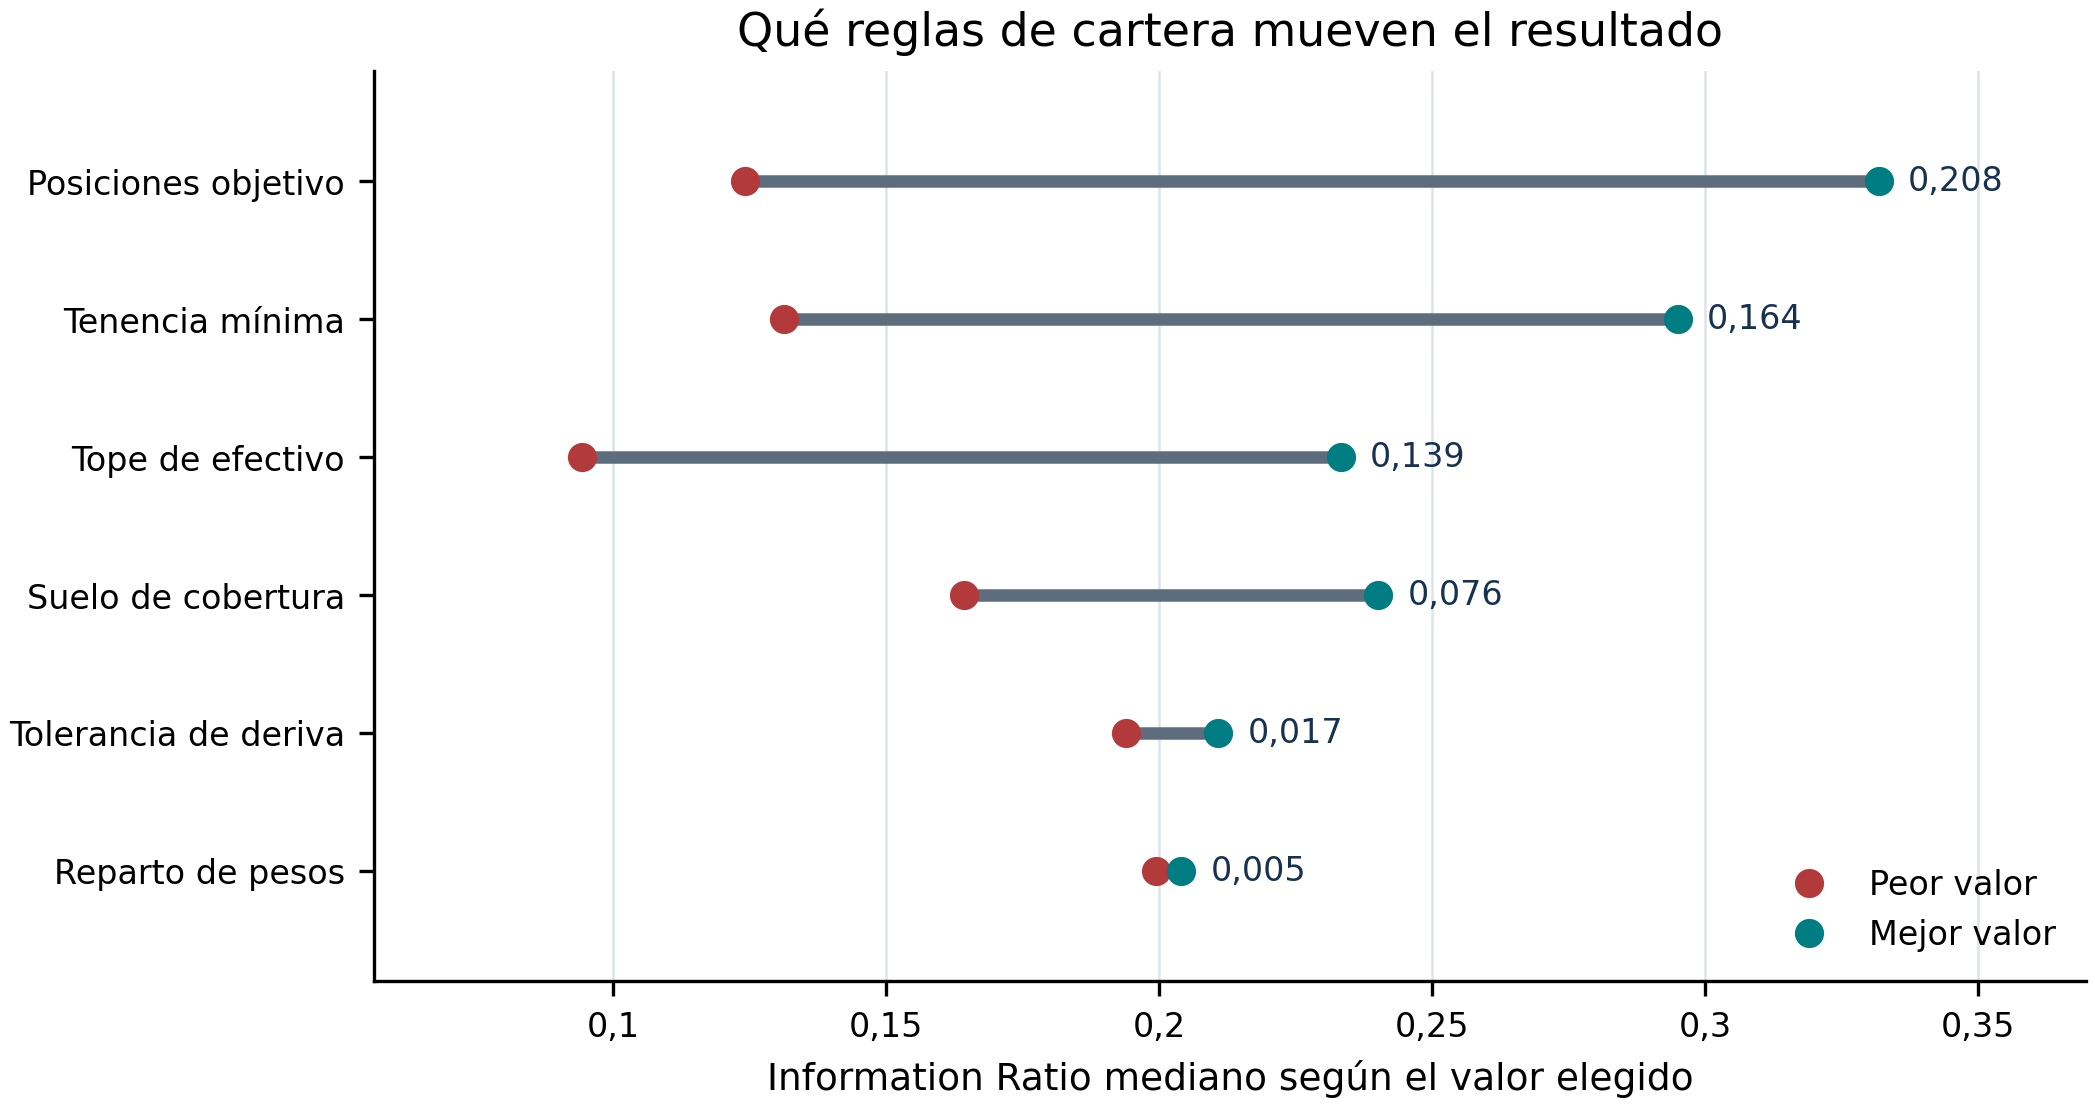
\includegraphics[width=\linewidth]{assets/f08_cartera_influencia.png}
    \end{column}
    \begin{column}{0.30\textwidth}
      {\large\textbf{Mueven más}}\\
      posiciones\\tenencia mínima\\efectivo\\[0.55cm]
      {\large\color{slate}\textbf{Mueven poco}}\\
      deriva\\reparto de pesos
    \end{column}
  \end{columns}
\end{frame}
\note{[0:55] La figura compara la mejor y peor mediana de IR para cada regla, dejando variar las
otras cinco. El número de posiciones mueve 0,208; la tenencia 0,164 y el efectivo 0,139. La deriva y
el reparto de pesos son casi inertes. Esto responde al objetivo 2a con toda la rejilla.}

% 14 · 0:55
\begin{frame}{\NumCarteras{} carteras revelan cuánto pesa la implementación}
  \begin{columns}[c,onlytextwidth]
    \begin{column}{0.66\textwidth}
      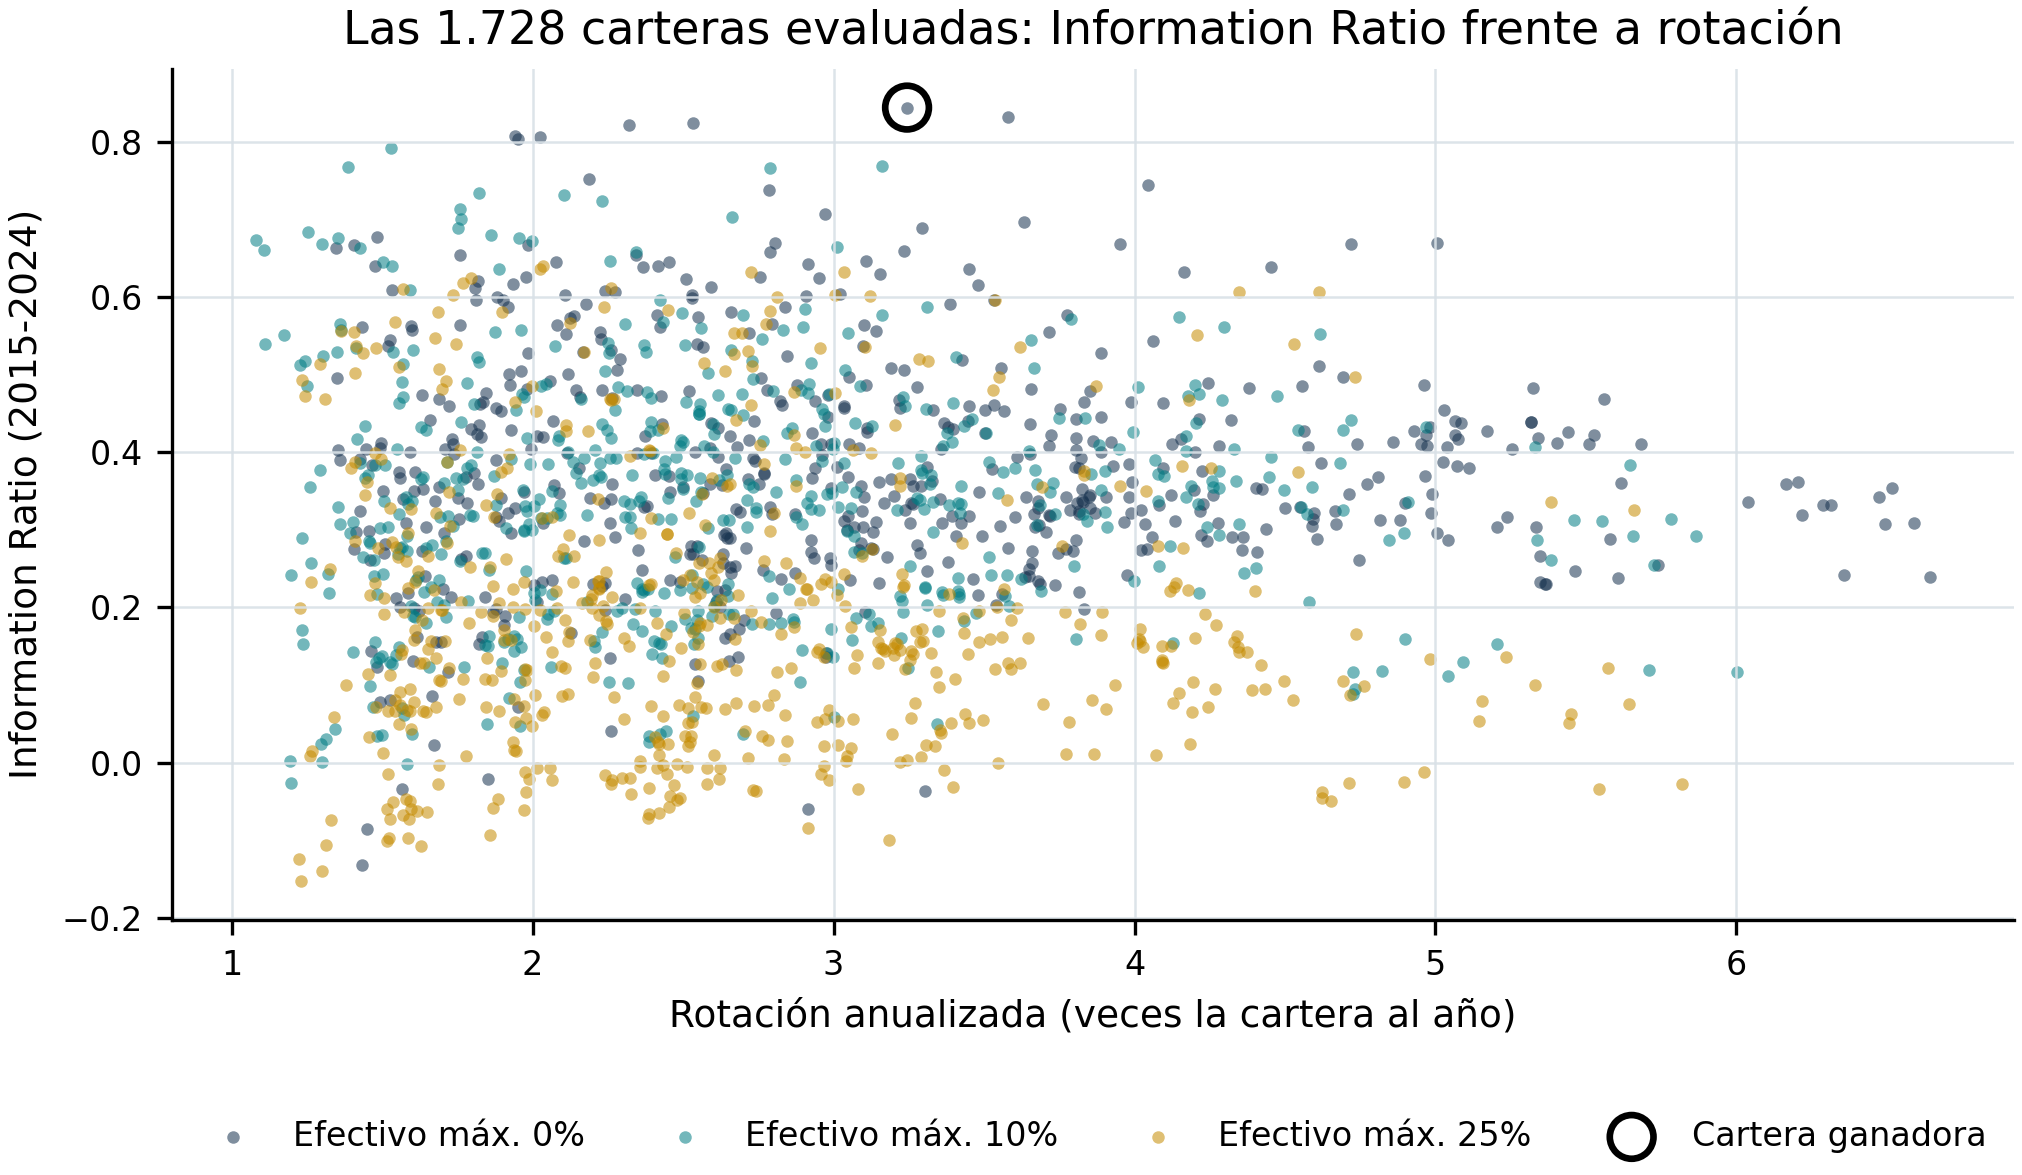
\includegraphics[width=\linewidth]{assets/f08_cartera_rejilla.png}
    \end{column}
    \begin{column}{0.30\textwidth}
      \cifra{\IRModelo{} $\rightarrow$ \IRCartera{}}{Information Ratio}
      \vspace{0.25cm}
      \cifra{\ExcesoModelo{} $\rightarrow$ \ExcesoCartera{}}{exceso geométrico}
    \end{column}
  \end{columns}
  \matiz{La cifra de la ganadora es optimista; la dispersión de toda la nube es el hallazgo robusto.}
\end{frame}
\note{[0:55] Cada punto cambia solo las seis reglas de cartera. La amplia dispersión vertical prueba
que la implementación altera el resultado. La rejilla es cartesiana porque las reglas interactúan;
elegir cada variable por separado no habría encontrado la combinación final.}

% 15 · 1:10
\begin{frame}{La ganadora opera menos y mejora dentro de selección}
  \small
  \begin{center}
  \begin{tabular}{lrrr}
    \toprule
    Métrica & Modelo & Ganadora & Reservada \\
    \midrule
    Information Ratio & \IRModelo{} & \textbf{\IRCartera{}} & \IRCarteraReservado{} \\
    Exceso geométrico & \ExcesoModelo{} & \textbf{\ExcesoCartera{}} & \ExcesoCarteraReservado{} \\
    Rotación anual & \TurnoverModelo{} & \textbf{\TurnoverCartera{}} & \TurnoverCarteraReservado{} \\
    Máxima caída & \MDDModelo{} & \textbf{\MDDCartera{}} & \MDDCarteraReservado{} \\
    \bottomrule
  \end{tabular}
  \end{center}
  \vspace{0.4cm}
  {\large\textbf{Política:} \PosicionesCartera{} posiciones · efectivo \EfectivoModelo{} $\to$
  \EfectivoCartera{} · tenencia medio horizonte $\to$ horizonte completo · deriva
  \DerivaModelo{} $\to$ \DerivaCartera{}.}
\end{frame}
\note{[1:10] La comparación usa la configuración real del Model Study: ya tenía media ventana de
tenencia mínima. La ganadora no cambia el número de posiciones ni el reparto proporcional al alfa.
Baja efectivo, alarga la tenencia y tolera más deriva. Las tres decisiones reducen la reacción y la
rotación cae casi a la mitad.}

% 16 · 1:05
\begin{frame}{El resultado se concentra en pocos nombres}
  \begin{center}
    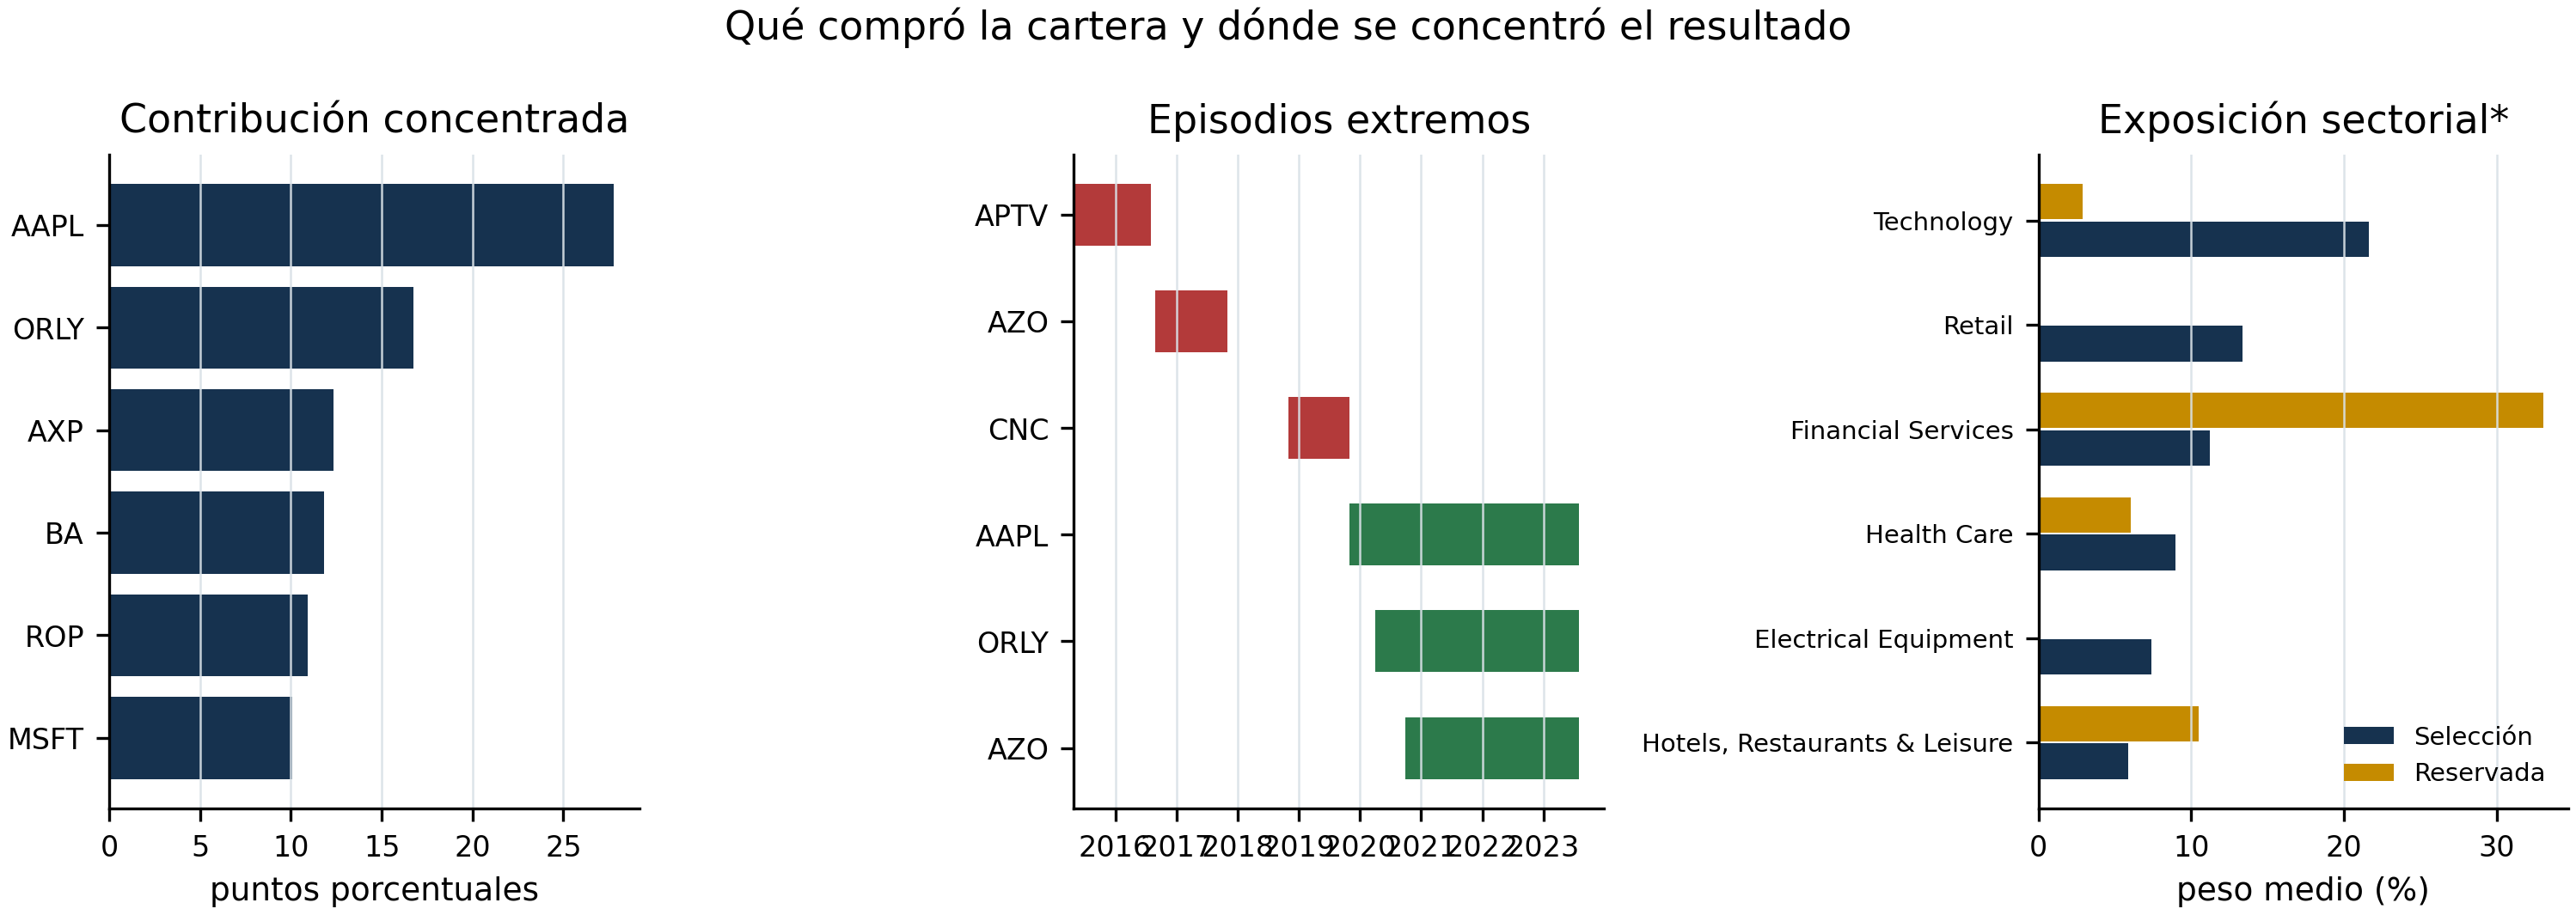
\includegraphics[width=0.94\linewidth]{assets/f07_cartera_narrativa.png}\\[-0.05cm]
    {\large\color{navy}
      \textbf{\NumAccionesCartera{} acciones} \quad·\quad
      \textbf{\MedianaMesesTenencia{} meses} de mediana \quad·\quad
      AAPL aporta \textbf{\ContribucionAAPL{}}}
  \end{center}
  \matiz{El sector es descriptivo y actual; no es una variable ni una clasificación point-in-time.}
\end{frame}
\note{[1:05] La cartera mantuvo 42 nombres en 49 episodios y una mediana de 15 meses. AAPL aporta
27,8 puntos acumulados, por lo que el resultado no está igualmente repartido. Las operaciones AAPL
y AZO explican por qué una tenencia mínima puede evitar ventas prematuras, sin convertir casos vistos
a posteriori en nuevas reglas.}

% 17 · 1:10
\begin{frame}{La optimización cambia el signo, pero aún no demuestra generalización}
  \vspace{-0.19cm}
  \begin{columns}[c,onlytextwidth]
    \begin{column}{0.55\textwidth}
      \centering
      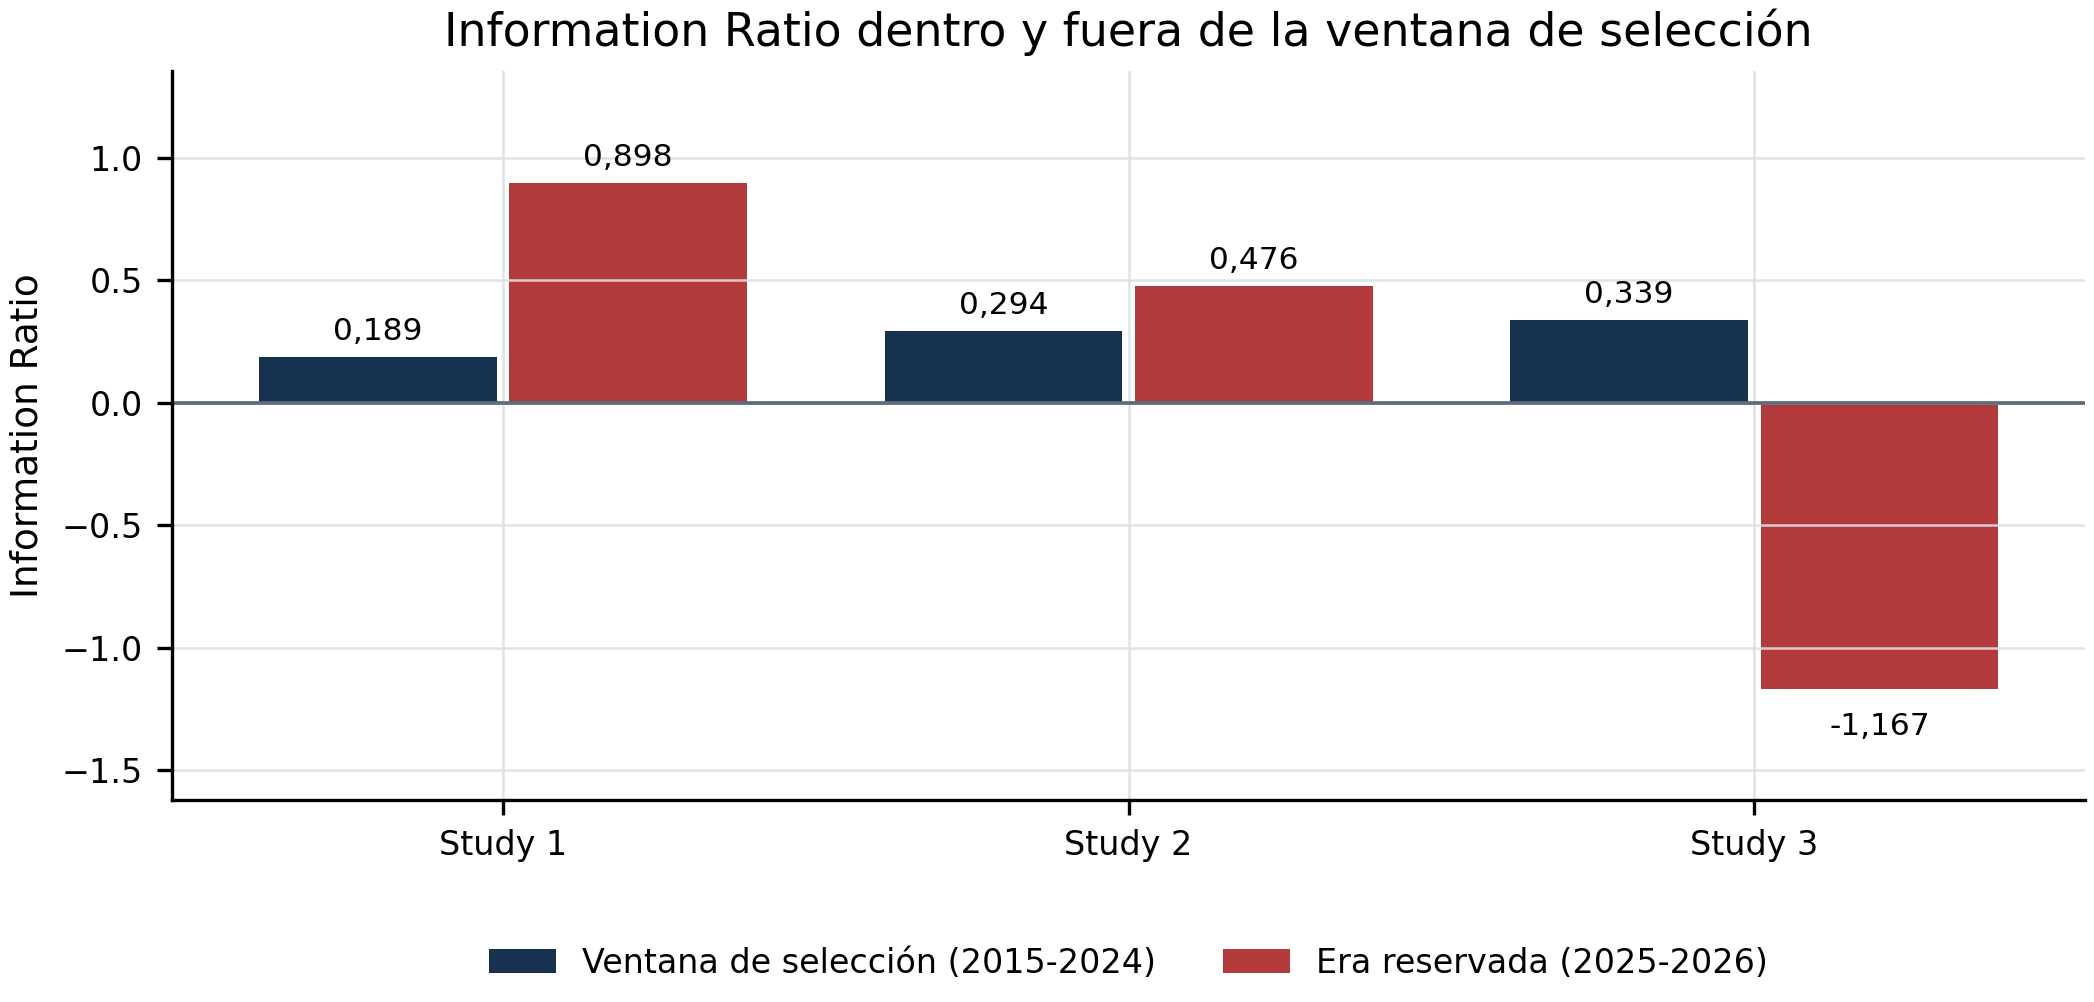
\includegraphics[width=0.90\linewidth]{assets/f09_seleccion_vs_reservada.png}
    \end{column}
    \begin{column}{0.41\textwidth}
      \cifracolor{\ExcesoModeloReservado{}}{cartera original}{rojo}
      \vspace{0.18cm}
      \cifracolor{\ExcesoCarteraReservado{}}{cartera optimizada}{verde}
      \vspace{0.18cm}
      \cifra{\RankICReservado{}}{misma señal en ambos casos}
    \end{column}
  \end{columns}
  \vspace{-0.19cm}
  \matiz{\CohortesReservadas{} cohortes y \AnosCarteraReservada{} años: evidencia preliminar, no validación económica.}
\end{frame}
\note{[1:10] Con la cartera original, la señal pierde 12,23 por ciento e IR menos 1,795. Con la
optimizada, mismo ranking y sin reentrenar, el exceso pasa a 0,24 e IR 0,109. Cambia el signo, no la
escala: es compatible con empatar. La rejilla demuestra que la cartera importa; este único periodo
no demuestra que la ganadora generalice.}

% 18 · 0:55
\begin{frame}{Los perfiles muestran sensibilidad, no una clasificación de estilos}
  \vspace{-0.25cm}
  \begin{center}
    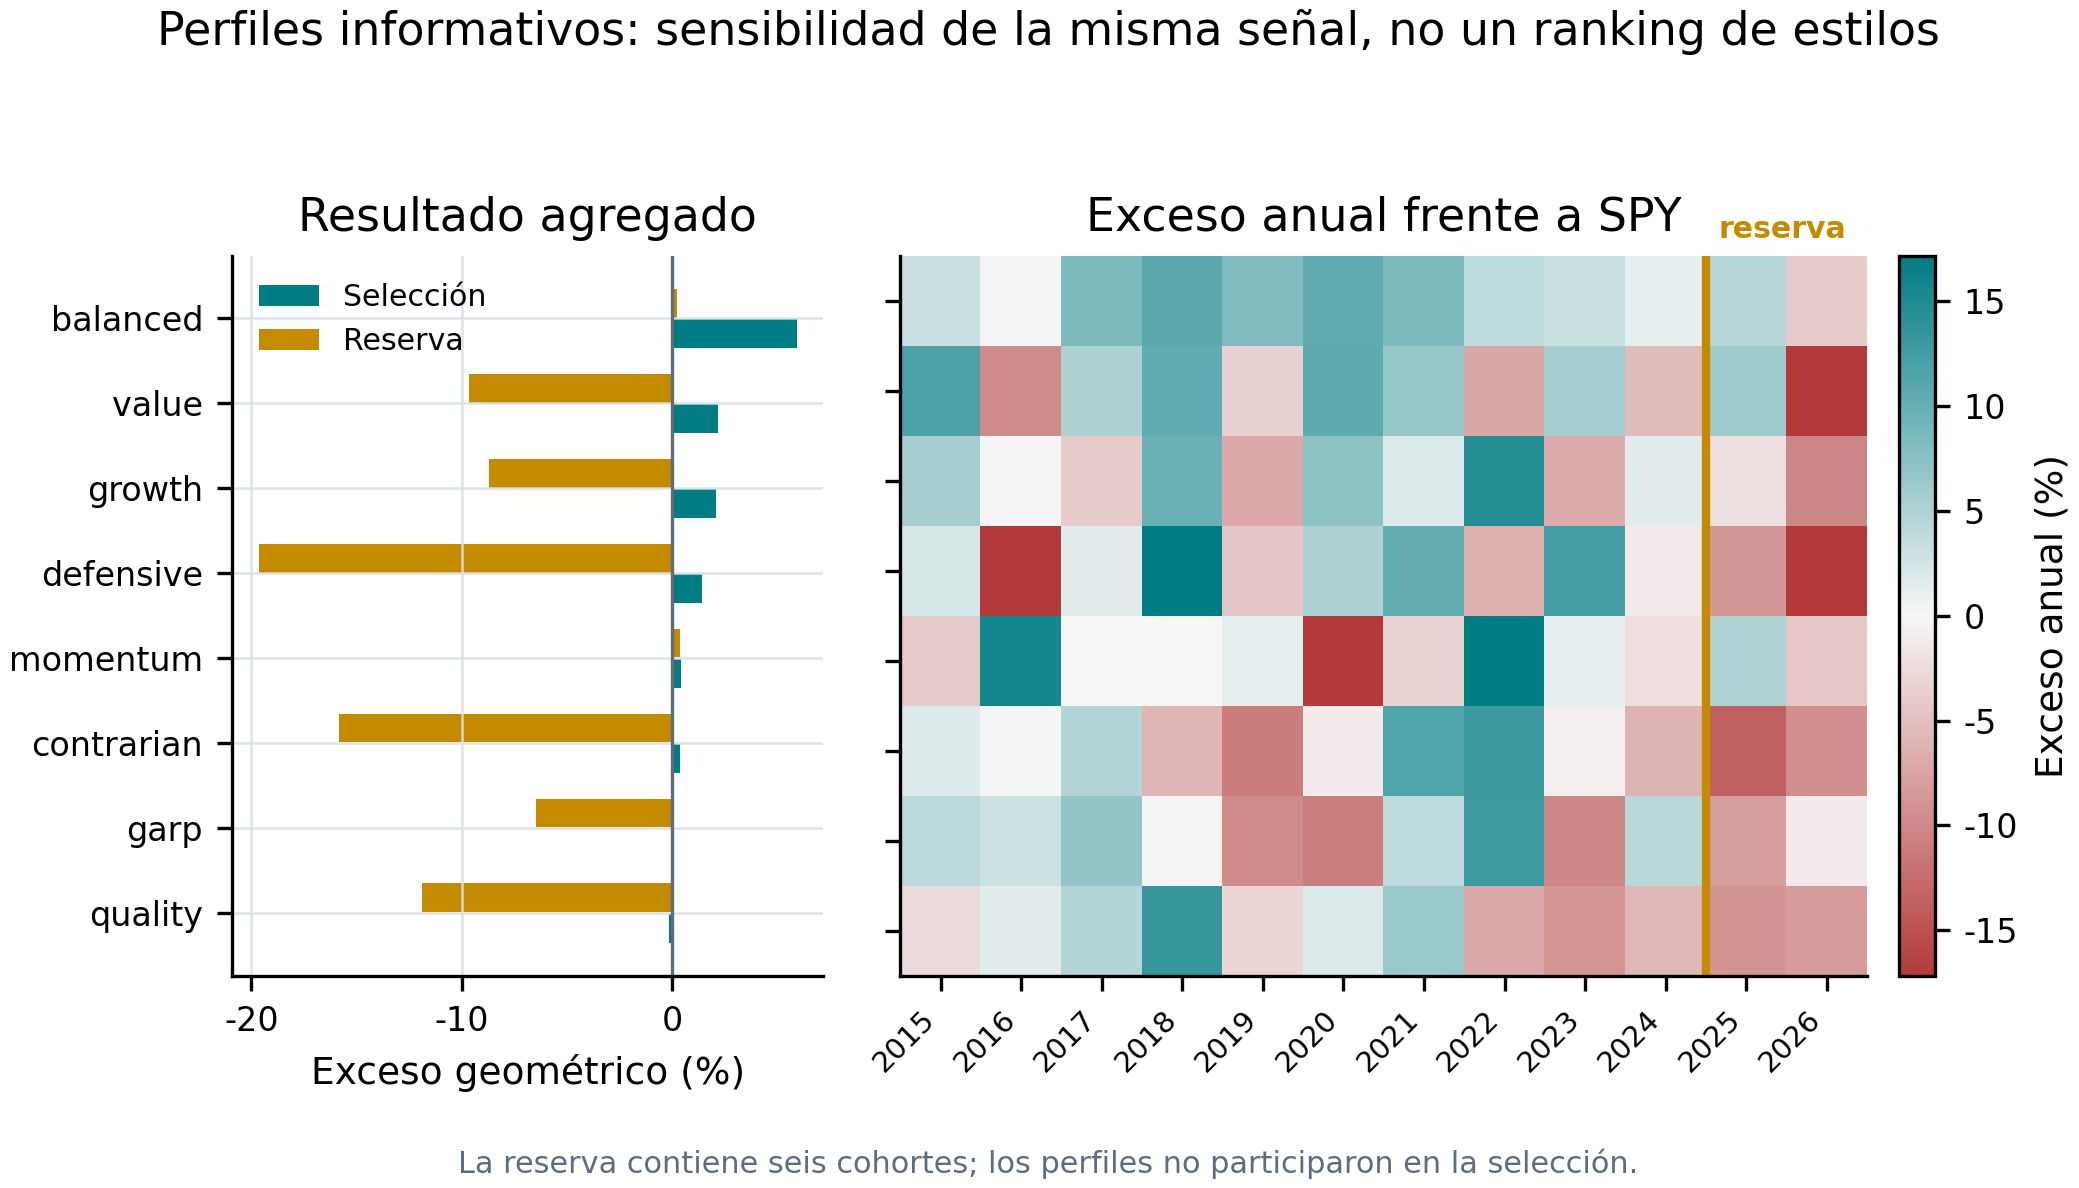
\includegraphics[width=0.74\linewidth]{assets/f07_perfiles_resultados.png}
  \end{center}
\end{frame}
\note{[0:55] Los ocho perfiles no reentrenan el modelo: reordenan las acciones que la señal ya
considera buenas. Balanced, que conserva el meta puro, domina en selección. En reserva solo balanced
y momentum mantienen un exceso ligeramente positivo, pero hay seis cohortes: el mapa sirve para ver
sensibilidad al estilo, no para ordenar ocho estrategias ni elegir una retrospectivamente.}

% 19 · 1:15
\setacto{navy}
\begin{frame}{Qué queda demostrado y qué no}
  \vspace{0.25cm}
  \begin{columns}[t,onlytextwidth]
    \begin{column}{0.30\textwidth}
      {\color{navy}\Large\textbf{1}}\\[0.25cm]
      {\large Ordenación favorable y robusta.}\\[0.3cm]
      {\color{slate}Sin demostrar la necesidad de cinco agentes.}
    \end{column}
    \begin{column}{0.30\textwidth}
      {\color{teal}\Large\textbf{2a}}\\[0.25cm]
      {\large Las reglas de cartera importan.}\\[0.3cm]
      {\color{slate}Demostrado sobre toda la rejilla.}
    \end{column}
    \begin{column}{0.30\textwidth}
      {\color{gold}\Large\textbf{2b}}\\[0.25cm]
      {\large La reserva es solo direccional.}\\[0.3cm]
      {\color{slate}No confirma generalización económica.}
    \end{column}
  \end{columns}
  \vspace{0.85cm}
  \begin{center}
    \colorbox{light}{\parbox{0.92\linewidth}{\centering\large
      Ninguna afirmación práctica sobre una señal es interpretable\\
      \textbf{sin declarar con qué cartera se midió}.}}
  \end{center}
\end{frame}
\note{[1:15] La contribución es metodológica. Una buena señal puede parecer inútil con una cartera
inadecuada, y una buena cartera puede maquillar una señal débil. Este trabajo separa selección,
robustez e implementación. El objetivo uno queda apoyado; el 2a, demostrado por la dispersión de
1.440 carteras; y el 2b sigue siendo preliminar por selección, multiplicidad y tamaño muestral.}

% 20 · 0:20 — total objetivo 18:15
{\setbeamertemplate{footline}{}
\begin{frame}[plain]
  \vspace{2.0cm}
  \hspace*{0.55cm}\begin{minipage}{0.88\linewidth}
    {\color{navy}\rule{2.2cm}{2pt}}\\[0.8cm]
    {\fontsize{28}{32}\selectfont\color{navy}\textbf{Gracias}}\\[0.65cm]
    {\large\textbf{Adrián Núñez}}\\[0.2cm]
    {\small\color{slate}Preguntas}
  \end{minipage}
\end{frame}}
\note{[0:20] Muchas gracias. Quedo a vuestra disposición para preguntas.}

% Reserva · sin numeración
{\setbeamertemplate{footline}{}
\begin{frame}[plain,noframenumbering]{Reserva · Cómo se construyen los perfiles}
  \vspace{-0.15cm}
  \begin{center}
    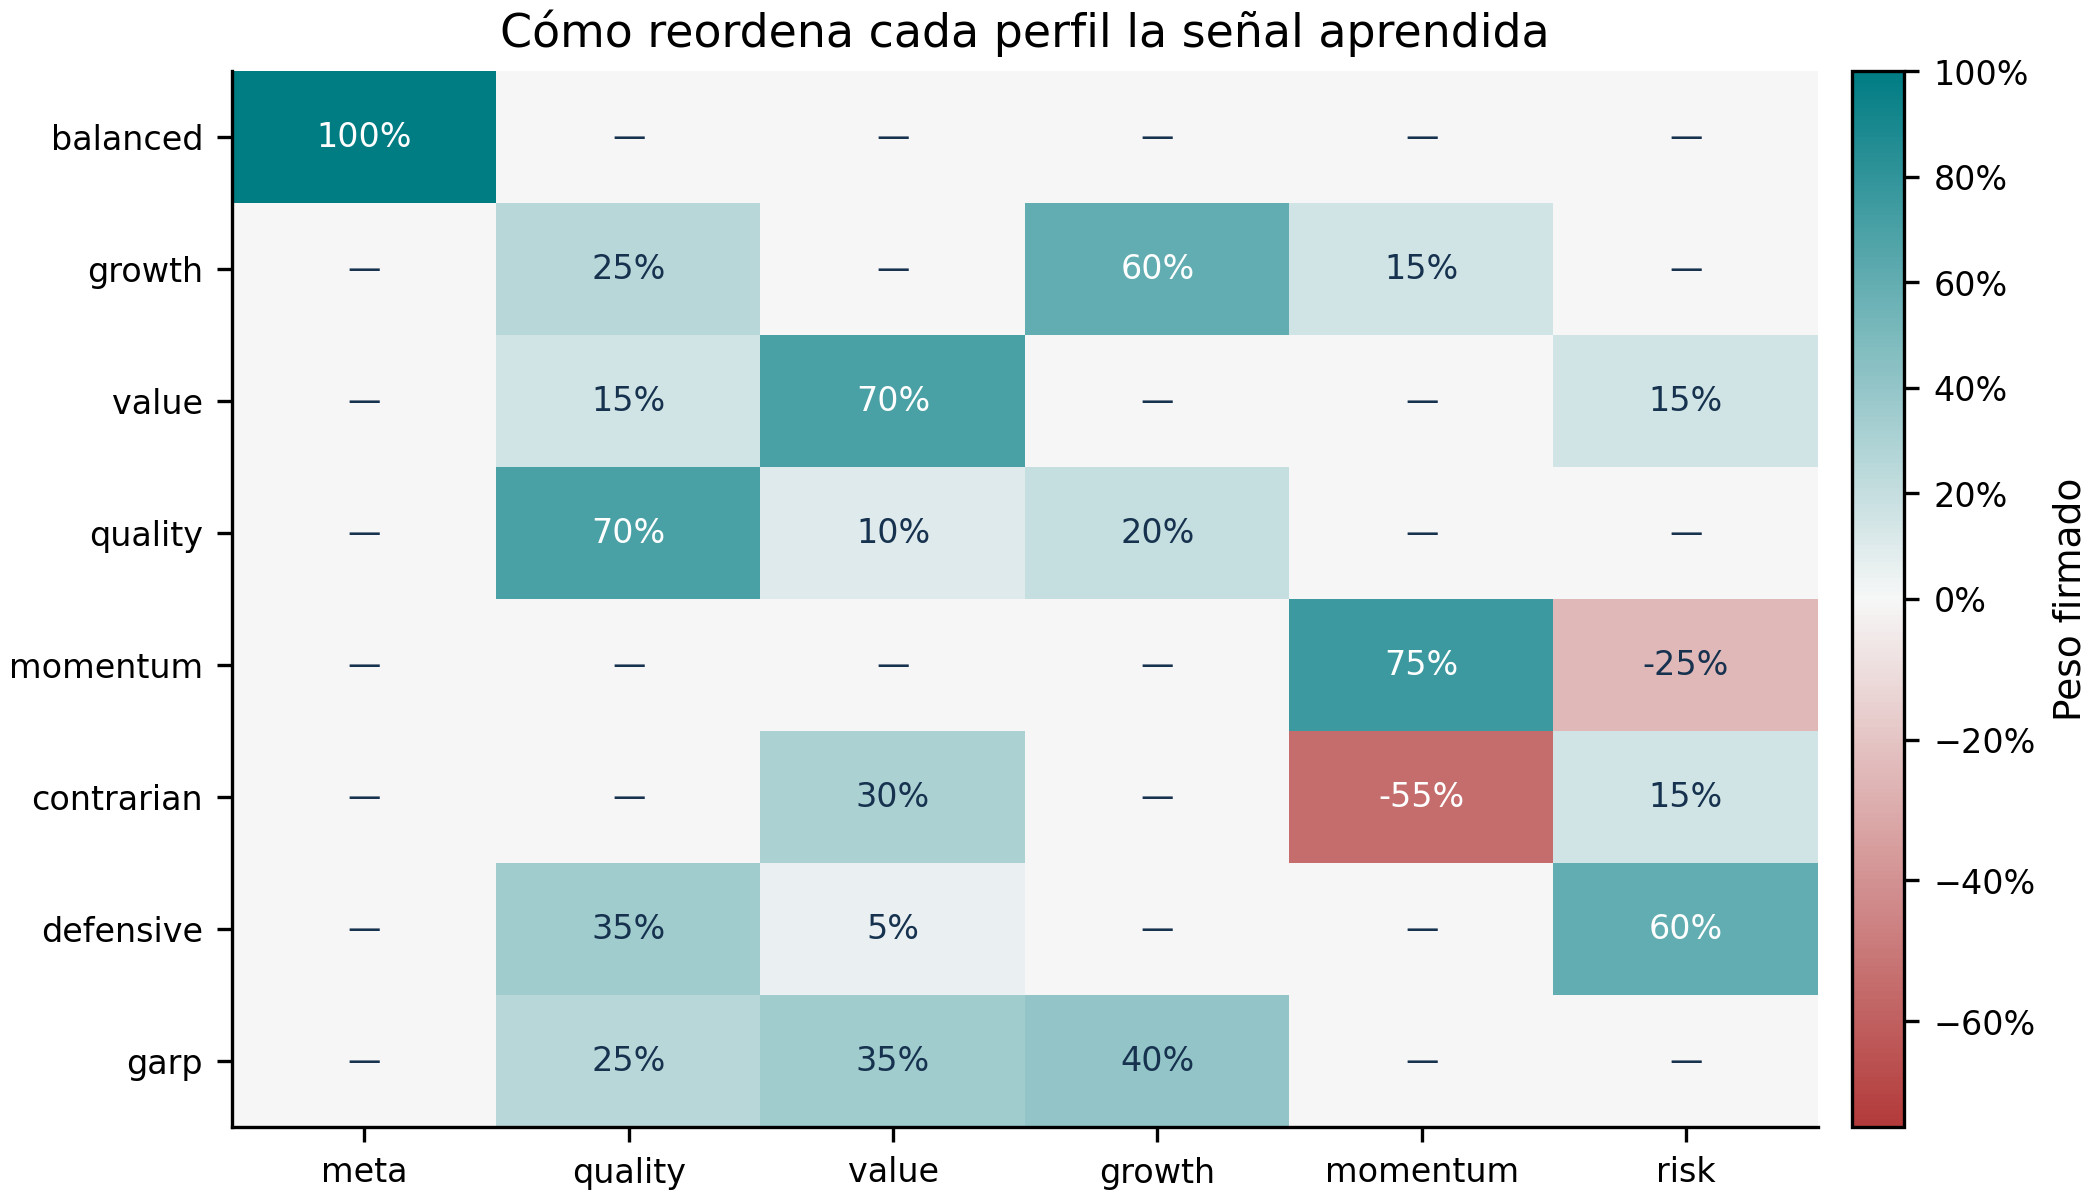
\includegraphics[height=0.78\textheight,keepaspectratio]{assets/f07_perfiles_pesos.png}
  \end{center}
\end{frame}}
\note{Diapositiva de reserva. Balanced es meta puro; los demás perfiles aplican pesos fijos y
firmados. Los pesos negativos hacen explícita una inclinación contra momentum o contra riesgo.}

\end{document}
